\documentclass{article}


\usepackage{arxiv}
\usepackage{mathptmx}
\usepackage[utf8]{inputenc} % allow utf-8 input
\usepackage[T1]{fontenc}    % use 8-bit T1 fonts
\usepackage{hyperref}       % hyperlinks
\usepackage{url}            % simple URL typesetting
\usepackage{booktabs}       % professional-quality tables
\usepackage{amsfonts}       % blackboard math symbols
\usepackage{nicefrac}       % compact symbols for 1/2, etc.
\usepackage{microtype}      % microtypography
\usepackage{lipsum}
\usepackage{enumitem}
\usepackage[polish]{babel}  % English language hyphenation
\usepackage{float}          % for H in \begin{figure}[H]. Force including file in place.
\usepackage{caption}
\usepackage{subcaption}
\usepackage{placeins}
\usepackage{graphicx}
\usepackage{lmodern}
\usepackage{adjustbox}
\usepackage{amsmath}

\graphicspath{./images/}

\usepackage{multirow}
\usepackage{booktabs}

\usepackage{caption}
\captionsetup[table]{skip=10pt}

\usepackage{titlesec}
\titlelabel{\thetitle.\quad}

%\fancyhf{} % sets both header and footer to nothing
\renewcommand{\headrulewidth}{0pt}
\AtBeginDocument{%
  \renewcommand\tablename{Tabela}
}
% your new footer definitions here

\newcommand{\todo}[1]{\textcolor{red}{TODO: #1}}

% kolory odnośników
\usepackage[dvipsnames]{xcolor}
\hypersetup{
    colorlinks=true,
    linkcolor=black,
    filecolor=black,
    citecolor=black,
    urlcolor=cyan,
    pdftitle={Sharelatex Example},
    pdfpagemode=FullScreen,
}
\urlstyle{same}


\title{Kwantyzacja wektorowa}

\author{
  Karol Działowski \\
  \textbf{Wojciech Olejnik} \\
  \textbf{Paweł Kalicki} \\
  Zachodniopomorski Uniwersytet Technologiczny
}

\begin{document}
\maketitle
\begin{abstract}
Problem kompresji plików multimedialnych jest kluczowy w akwizycji, przechowywaniu i przesyłaniu takiego rodzaju danych. Większośc multimediów z jakimi mamy do czynienia jest poddawana kompresji.

W ramach zajęć Zespołowy projekt badawczy 2 zaimplementowano algorytm kompresji bazujący na kwantyzacji wektorowej oraz stworzono raport opisujący podstawy teoretyczne zaproponowanego rozwiązania. 

W procesie kompresji wykorzystywana jest kwantyzacja wektorowa z usuniętymi średnimi. Słownik służący kwantyzacji zbudowany jest za pomocą algorytmu LBG. Usunięte średnie z kwantyzacji wektorowej zostały poddane kompresji przy użyciu kodowania różnicowego i koderu Golomba.

Podczas realizacji projektu przeprowadzono badania dotyczące pojedynczych elementów zaproponowanej kompresji. Zaproponowany algorytm jest gorszy od standardu JPEG pod względem podobieństwa do obrazu oryginalnego porównanego zgodnie z metryką PSNR dla takich samych współczynników kompresji.
\end{abstract}

\newpage

\tableofcontents

\newpage

% keywords can be removed
%\keywords{First keyword \and Second keyword \and More}


\section{Wstęp}

Kompresja danych multimedialnych ma ogromne znaczenia w dobie internetu. Rozwój algorytmów kompresji nie jest jednak zakończony. Tymi zagadnieniami zajmują się nie tylko naukowcy ale także inżynierowie z światowych marek technologicznych z branż takich jak streaming wideo, produkcji sprzętu czy twórcy systemów operacyjnych \cite{intel}.

W tej pracy zajmować się będziemy kompresją obrazów w odcieni szarości. Istnieje wiele metod kompresji, które mają ugruntowaną pozycję na rynku. Są to między innymi standard JPEG, PNG czy WebP \cite{ginesu2012objective}. Nasze podejście polegać będzie na wykorzystaniu kwantyzacji i innych pomocniczych algorytmów które będą połączone w cały proces kompresji stratnej.

Kwantyzacja polega na przyporządkowaniu wartościom sygnału ciągłego wartości dyskretnych należących do skończonego zbioru.
Przedział wartości sygnału dzielony jest na zbiór przedziałów.
Zazwyczaj przedziały mają taką samą wielkość (kwantyzacja liniowa).
Stosuje się też kwantyzację nieliniową, gdzie przedziały nie są równomiernie podzielone.

Z każdym przedziałem powiązany jest określony poziom kwantyzacji.
Gdy wartość sygnału wejściowego należy do danego przedziału przyporządkowuje mu się odpowiednią wartość kwantyzacji.

Podczas procesu kwantyzacji powstają błędy kwantyzacji wynikające z różnicy rzeczywistej wartości od wartości kwantyzacji.
Błędy te objawiają się w postaci tak zwanego szumu kwantyzacji.
Im większe przedziały kwantyzacji tym mniejsza jej dokładność i tym większy jest szum kwantyzacji.
W przetwarzaniu analogowo-cyfrowym dokładność liniowej kwantyzacji jest określona przez liczbę bitów wykorzystywanych do zapisu skwantyzowanej wartości.
Zwiększenie liczby bitów prowadzi do zwiększenia liczby przedziałów, co w rezultacie prowadzi do dokładniejszego odwzorowania \mbox{sygnału \cite{drozdek2007wprowadzenie}.}

\section{Opis projektu}
\label{sec:opis}

Celem projektu było stworzenie aplikacji umożliwiającej przeprowadzanie kwantyzacji wektorowej oraz przeprowadzenie badań
zaimplementowanych metod. 

Podczas zajęć stworzono rozwiązanie end-to-end, które realizuje kompresję obrazów w skali szarości wykorzystując kwantyzację wektorową z usuniętymi średnimi \cite{meanremovedVQ}, algorytm budowy słownika LBG \cite{lbg1980} oraz kodowanie różnicowe \cite{differential_coding} i koder Golomba \cite{golomb}. Oprócz kompresji do pliku zaimplementowano etap rekonstrukcji obrazu z kodu binarnego udowadniając poprawność działania procesu kompresji.

W rozdziale trzecim wyłożono teorię potrzebną do implementacji wykorzystanych metod. Rozdział czwarty przedstawia badania empiryczne na zaimplementowanych metodach i algorytmach. 

Praca została wykonana na kursie \emph{Zespołowy projekt badawczy 2} w semestrze zimowym 2020/21. Kod źródłowy tego raportu oraz zaimplementowanych metod i przeprowadzonych badań dostępny jest pod adresem \url{https://github.com/karlosos/image_vector_quantization}.

\subsection{Metodologia pracy}

W ramach zespołu dokonaliśmy podziału pracy zgodnie z trzema rolami. Pierwszą z nich była rola dokumentalisty, która polegała na zbieraniu i opracowywaniu materiałów w postaci tego dokumentu. Druga rola to ,,zdobywacz wiedzy'', która w założeniu miała za zadania akwizycję wiedzy i jej przekazywanie pozostałym członkom zespołu. Trzecia rola to klasyczny programista mający za zadanie implementację opracowanych algorytmów.

Podział ról wyglądał następująco:

\begin{itemize}
    \item Karol Działowski -- programista i dokumentalista,
    \item Wojciech Olejnik -- dokumentalista i zdobywacz wiedzy,
    \item Paweł Kalicji -- programista i zdobywacz wiedzy.
\end{itemize}

W przypadku naszego zespołu taki podział ról się nie sprawdził i nie był ściśle przestrzegany. Do podziału pracy w ramach zespołu wykorzystano podejście elastyczne. Opierało się na transparentnym spisie zadań na współdzielonej tablicy, gdzie po każdych zajęciach dodawano nowe zadania. Ponadto jeden z członków zespołu był odpowiedzialny za integrację całego projektu, kontakt z prowadzącym oraz kontrolę nad współdzieloną tablicą.

Rola ,,zdobywacza wiedzy'' w praktyce nie była realizowana. Materiały niezbędne do implementacji w większości były dostarczane nam przez prowadzącego. Dodatkowo próbowaliśmy pomijać wymianę wiedzy pomiędzy członkami zespołu, co mogło przełożyć się na mniejszą produktywność zespołu.

\section{Wstęp teoretyczny}

W tym rozdziale przedstawione zostały opisy teoretyczne wykorzystanych metod w procesie kompresji. Głównym elementem naszej pracy jest kwantyzacja wektorowa.

\subsection{Kwantyzacja wektorowa}
Kwantyzacja wektorowa (ang. \emph{vector quantization}) polega na podziale wielowymiarowych przestrzeni na obszary i
przyporządkowanie każdemu obszarowi odpowiedniego poziomu kwantyzacji.
Obszary reprezentowanego są w formie wektorów.
Jednym z zastosowań kwantyzacji wektorowej jest kompresja obrazów.

W celu kwantyzacji obraz dzielony jest na obszary o zadanym rozmiarze, np. $4 \times 4$ pikseli, co tworzy wektory o długości $16$.
Budowana jest książka kodowa reprezentująca poziomy kwantyzacji na podstawie wyznacznych wektorów.
Dla każdego obszaru detekcyjnego przyporządkowuje się indeks wyznaczonego najbliższego poziomu kwantyzacji. Przykład podziału dwuwymiarowej przestrzeni danych na klastry przedstawiono na rysunku (\ref{fig:kwantyzacja_wektorowa}).

Jakość kwantyzacji zależy od długości wektorów i doboru książki kodowej. Na jakość książki kodowej wpływa proces jej budowy oraz liczba elementów w książce kodowej.

\begin{figure}[h]
  \centering
  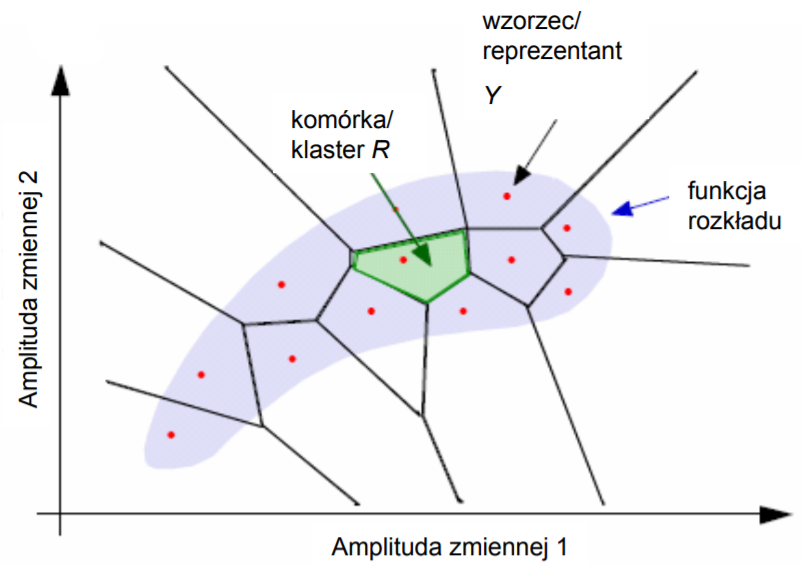
\includegraphics[width=0.6\textwidth]{images/kwantyzacja_wektorowa.png}
  \caption{Przykład podziału dwuwymiarowej przestrzeni danych na klastry grupujące według słownika. Źródło \cite{mwilczewski}.}
  \label{fig:kwantyzacja_wektorowa}
\end{figure}

\subsection{Ogólny przebieg etapów pracy kwantyzatora wektorowego}

\begin{enumerate}
  \item Formowanie danych wejściowych do postaci $K$ wektorów $v$ -- wymiarowych (etap wstępny).
  \item Faza klasteryzacji: podział wszystkich wektorów wejściowych i konstrukcja książki
        kodowej (słownika) zawierającej $p$ najbardziej reprezentatywnych wektorów całego zbioru danych,
        tzw. wektorów kodowych. Konstrukcja książki kodowej może być wykonana w fazie wstępnej na podstawie zbioru
        treningowego lub dynamicznie we właściwej fazie kwantyzacji. Faza klasteryzacji jest kluczowym etapem kwantyzacji wektorowej.
  \item Faza indeksowania: przyporządkowanie każdemu wektorowi wejściowemu jednego wektora ze słownika i reprezentowanie wektora wejściowego indeksem słownika. Etap przedstawiono na rysunku (\ref{fig:wektory_danych}).
\end{enumerate}

Ogólny schemat kwantyzacji przedstawiono na rysunku (\ref{fig:schemat_kwantyzatora}).

\begin{figure}[h]
  \centering
  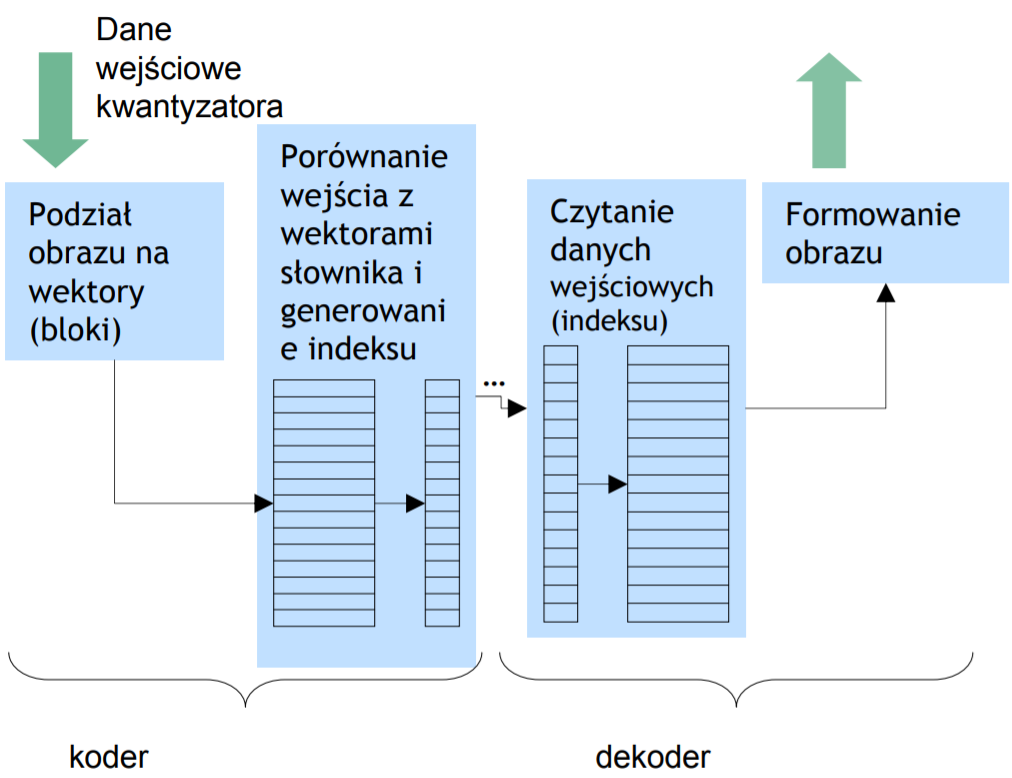
\includegraphics[width=0.6\textwidth]{images/schemat_kwantyzatora.png}
  \caption{Ogólny schemat pracy kwantyzatora. Źródło \cite{mwilczewski}.}
  \label{fig:schemat_kwantyzatora}
\end{figure}

\begin{figure}[h]
  \centering
  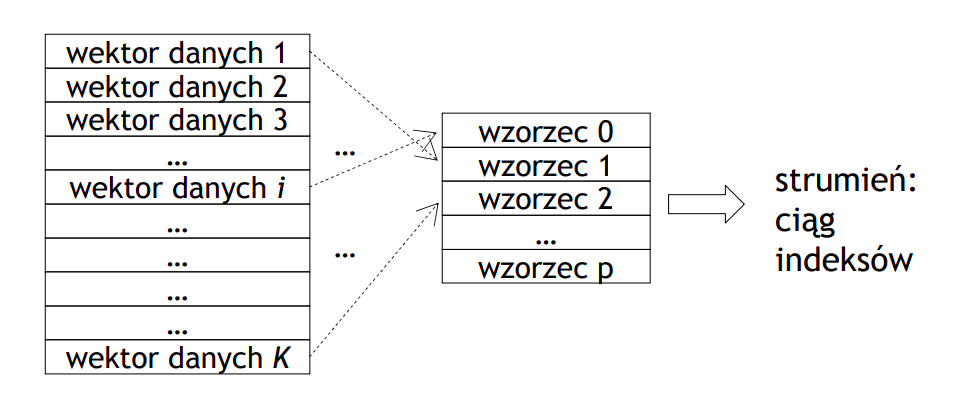
\includegraphics[width=0.6\textwidth]{images/wektory_danych.png}
  \caption{Porównywanie wektorów danych z wektorami ze słownika. Źródło \cite{mwilczewski}.}
  \label{fig:wektory_danych}
\end{figure}

Problemy jakie możemy napotkać podczas kwantyzacji wektorowej:
\begin{enumerate}
  \item Wybór odpowiedniej funkcji odległości w przestrzeni wektorowej.
  \item Struktura książki kodowej (prosta struktura w postaci tablicy jest nieefektywna do przeglądania).
\end{enumerate}

\paragraph{Sparametryzowany wzór pliku wynikowego}
\label{sec:lgb_file_size}
Plik wynikowy kwantyzacji wektorowej składa się ze słownika o określonej długości $K$ oraz wartości przyporządkowanych indeksów do każdego bloku. Każdy element słownika reprezentowany jest przez wektor o długości $v$, który zapisywany jest na $v \cdot 8$ bitach.

Każdy blok jest opisywany przez indeks, który można zapisać na $\log_2(K)$ bitach. Przykładowo dla słownika $512$ elementowego każdy wektor będzie reprezentowany przez indeks zapisany na $9$ bitach.


Dla rozmiaru obrazu wejściowego $m \times n$ pikseli, długości słownika $K$ i wielkości wektora wyrażanej przez $v$ otrzymujemy słownik o rozmiarze

\begin{equation}
  \textrm{dict\_size} = K \cdot v \cdot 8 \quad \textrm{[bitów]}.
  \label{eq:lgb_dict_size}
\end{equation}

Każdy blok przechowujący indeks ma rozmiar:

\begin{equation}
  \textrm{block\_size} = \log_2(K)  \quad  \textrm{[bitów]}.
  \label{eq:lgb_indeks_size}
\end{equation}

Dla obrazie o wielkości $m \times n$ otrzymujemy $\frac{mn}{v}$ bloków. Cały obraz zapisany na: 

\begin{equation}
  \textrm{file\_size} = \textrm{dict\_size} + \frac{mn}{v} \cdot \textrm{block\_size}  \quad  \textrm{[bitów]}.
  \label{eq:lgb_image_size}
\end{equation}

\subsubsection{Kwantyzacja wektorowa z usuniętą średnią}

Kwantyzacja wektorowa z usuniętą średnią (ang. \emph{mean-removed vector quantization} (MRVQ)) jest zmodyfikowaną wersją schematu kwantyzacji wektorowej \cite{meanremovedVQ}.

Celem MRVQ jest zapewnienie lepszej jakości obrazu od klasycznej kwantyzacji. Jest to osiągane za pomocą dodatkowej informacji jaką jest wartość średnia piksela dla każdego bloku. Ceną takiego podejścia jest spadek stopnia kompresji ze względu na konieczność przechowywania dodatkowych 8 bitów przechowujących wartość średnią dla każdego bloku.

Schemat kwantyzacji wektorowej z usuniętą średnią jest analogiczny do klasycznej kwantyzacji wektorowej. Algorytm kodowania składa się z następujących kroków:

\begin{enumerate}
  \item Stworzenie bloków (wektorów) z obrazu wejściowego.
  \item Wyliczenie wartości średniej każdego bloku.
  \item Stworzenie bloków resztkowych poprzez usunięcie średniej od każdej wartości bloku.
  \item Budowa książki kodów resztkowych (ang. \emph{residual codebook} (RCB)) -- na przykład korzystając z algorytmu LBG.
  \item Skojarzenie z każdym blokiem resztkowym pary -- indeksu najbliższego wektora resztkowego z książki kodowej oraz średniej danego bloku.
\end{enumerate}

Wartość średnia bloku $bm$ dla każdego bloku obrazu $x$ i wektorów o długości $k$ jest obliczana za pomocą wyrażenia: 

\begin{equation}
  bm = \frac{1}{k} \sum_{i=0}^{k-1} x_{i},
\end{equation}

Źródło: \cite{meanremovedVQ}

Algorytm dekodowania składa się z następujących kroków:

\begin{enumerate}
  \item Przyporządkowanie każdemu blokowi obrazu opisanego przez parę (indeks, średnia) odpowiedniego bloku resztkowego przechowywanego w książce kodów resztkowych.
  \item Dodanie do każdego elementu odczytanego bloku przechowywaną wartość średnią.
\end{enumerate}

\paragraph{Sparametryzowany wzór na długość pliku wynikowego}

Plik wynikowy budowany jest analogicznie do pliku wynikowego przedstawionego w sekcji \ref{sec:lgb_file_size} z tą różnicą, że dla każdego bloku przechowującego indeks musimy przechowywać też usuniętą średnią, która zapisana jest na $8$ bitach.

Każdy blok przechowujący indeks ma rozmiar:

\begin{equation}
  \textrm{block\_size} = log_2(K) + 8 \quad  \textrm{[bitów]}.
  \label{eq:mrev_indeks_size}
\end{equation}

W związku z odejmowaniem wartości średniej od każdego piksela w bloku musimy brać pod uwagę przechowywanie liczb ujemnych. Z tego względu pojedynczy element wektora resztkowego zapisywany jest na 9 bitach względem 8 bitów w podejściu klasycznym. Zdefiniujmy nowy wzór na rozmiar słownika:

\begin{equation}
  \textrm{dict\_size} = K \cdot v \cdot 9 \quad \textrm{[bitów]}.
  \label{eq:mrvq_dict_size}
\end{equation}

Łącząc wzór na wielkość słownika w bitach (\ref{eq:mrvq_dict_size}) oraz wzór na reprezentację pojedynczego wektora w bitach (\ref{eq:mrev_indeks_size}) otrzymujemy:

\begin{equation}
  \textrm{file\_size} = \textrm{dict\_size} + \frac{mn}{v} \cdot \textrm{block\_size}  \quad  \textrm{[bitów]},
  \label{eq:mrvq_image_size}
\end{equation}

dla obrazu o rozmiarze $m \times n$ pikseli, długości słownika $K$ i wielkości wektora wyrażanej przez $v$.

\subsection{Inicjalizacja książki kodowej}

W procesie kwantyzacji wektorowej ważną rolę odgrywa proces inicjalizacji książki kodowej.
Ma to znaczenie w procesie budowy książki kodowej, gdzie efektywność zależy od początkowych wartości \cite{arthur2006k}.
Źle dobrane wartości inicjalizacyjne mogą przeszkadzać w zbieżności algorytmu.

Podstawowymi metodami inicjalizacji książki kodowej są:

\begin{enumerate}
  \item metoda losowania,
  \item metoda grupowania najbliższych sąsiadów (ang. PNN - pairwise nearest neighbour),
  \item metoda rozdzielania (ang. splitting).
\end{enumerate}

Metoda losowa polega na wylosowaniu $N$ wektorów, gdzie $N$ jest liczba całkowitą.
Rozwiązanie jest wykorzystywane gdy posiada się mało informacji na temat danych wektorowych lub liczy się
szybkość inicjalizaci.

Druga metoda tworzenie słownika, czyli metoda grupowania najbliższych sąsiadów pozwala osiągnąć lepsze wyniki niż metoda losowa,
ale za to jest dużo bardziej czasochłonna.
Polega ona na tworzeniu coraz liczniejszych grup zaczynając od jednoelementowej, związanej z każdym wektorem sekwencji.
W następnych iteracjach wyznaczamy najbliższe grupy, czyli liczymy odległości pomiędzy środkami poszczególnych grup.
Następnie dwie najbliższe sobie grupy zostają połączone tak aby zmniejszać liczbę grup.

Algorytm metody PNN:

\begin{enumerate}
  \item Rozważamy zestaw $N$ wektorów treningowych w przestrzeni euklidesowej $K$-wymiarowej.
        Zadaniem konstrukcji książki kodowej jest odnalezienie zestawu wektorów kodowych $M$ poprzez minimalizację średniej kwadratowej odległości $T_i$ pomiędzy wektorami treningowymi $M$, a ich reprezentatywnymi wektorami z książki kodowej $C_j$:
                \begin{equation}
          D = \frac{1}{N} \sum_{j=1}^M \sum_{T_{i}\in\mathbb{S_{j}}} ||T_{i} - C_{j}||^2
        \end{equation}

  \item $S=S_{1}$,...,$S_{m}$ definiuje grupowanie zestawu treningowego $T$.
        Dla danego kodeksu $C$.
        Optymalne grupowanie może być zbudowane poprzez przypisanie każdego wektora $T_{i}$ do klastra $j_{0}$ dla którego:

        \begin{equation}
          ||T_{i} - C_{j0}||^2 = \displaystyle \min_{j_1,\dots ,M} ||T_{i} - C_{j}||^2
        \end{equation}

  \item Metoda ta rozpoczyna się od zainicjowania każdego wektora szkoleniowego $T_{i}$ jako własny klaster $S_{i}$.
        Na każdym etapie algorytmu, dwa najbliższe klastry ($S_{a}$ i $S_{b}$) są przeszukiwane i łączone.
        Odległość (koszt połączenia) $d$ pomiędzy dwoma klastrami jest definiowany jako wzrost zniekształcenia książki kodowej w przypadku połączenia klastrów:

        \begin{equation}
          d(S_{a}, S_{b}) = \frac{n_{a}n_{b}}{n_{a} + n_{b}} || C_{a} - C_{b} ||^2
        \end{equation}

  \item Wybrane klastry $S_{a}$ i $S_{b}$ są następnie łączone. Wielkość połączonych klastrów $S_{a}$ i $S_{b}$ wynosi $n_{a+b} = n_{a} + n_{b}$,
        a odpowiednim wektorem kodu jest centroid wektorów szkoleniowych w klaster. Można go obliczyć jako średnią ważoną $C_{a}$ i $C_{b}$:

        \begin{equation}
          C_{a + b} = \frac{n_{a}C_{a} + n_{b}C_{b}}{n_{a} + n_{b}}
        \end{equation}
        
  \item Wystarczy zatem utrzymać tylko centroidy klastra $C_{i}$ i rozmiary klastrów $n_{i}$ w realizacji algorytmu.
        Proces łączenia jest powtarzany do momentu aż książka kodowa osiągnie rozmiar $M$. 
        
\end{enumerate}

gdzie:
\begin{itemize}[label=]
  \item $T$ - Zestaw $N$ wektorów treningowych $T = {[T_{1}, T_{2}, \dots, T_{N}]}$
  \item $C$ - Książka kodowa wektorów $C = {[C_{1}, C_{2}, \dots, C_{m}]}$
  \item $M$ - Rozmiar książki kodowej
  \item $K$ - Wymiar wektorów
  \item $S_{i}$ - Klaster (zestaw) wektorów treningowych $n_{i}$
  \item $NN_{i}$ - Indeksy najbliższego sąsiada klastra $S_{i}$
  \item $d_{i}$ - Zwiększenie zniekształcenia w przypadku połączenia klastrów $S_{i}$ i $NN_{i}$
        \cite{tkaukoranta}
\end{itemize}

Ostatnia wymieniona metoda jaką jest metoda rozdzielania polega na szukaniu optymalnej książki.
Konstrukcja rozpoczyna się od pojedynczego wektora – centroidu zbioru uczącego.
W $i$-tym kroku dokonywany jest (w drodze dodawania zaburzenia) podział każdego z wektorów kodowych na dwa wektory.
Po takim rozdzieleniu uzyskana konfiguracja regionów decyzyjnych jest optymalizowana przez algorytm LBG, po czym dokonywany jest kolejny rozdział, etc.

\begin{figure}[H]
  \centering
  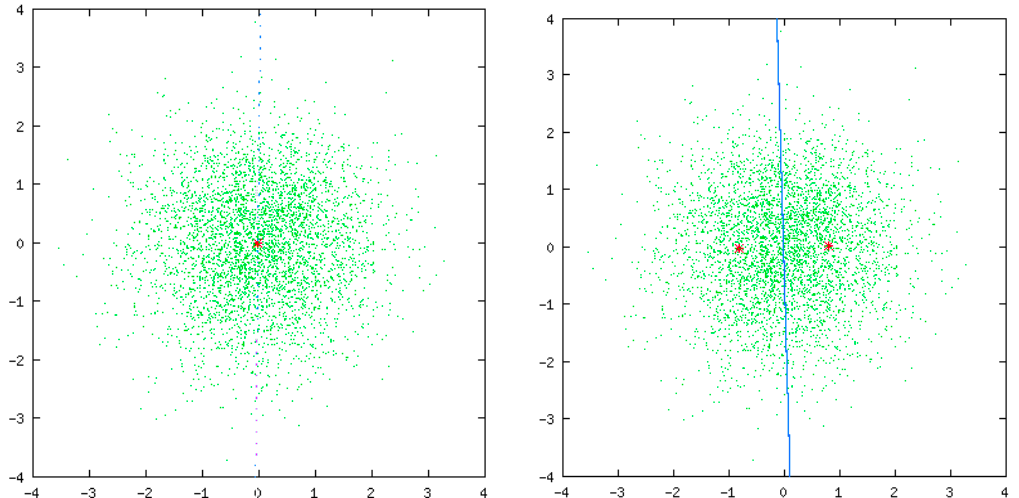
\includegraphics[width=0.6\textwidth]{images/rodzielania_1.png}
  \caption{Konstrukcja słownika metodą rozdzielania. Kolejne etapy konstrukcji wektorów kodowych
    (zaznaczone czerwonymi punktami) na zbiorze uczącym (zaznaczony kolorem zielonym). Źródło \cite{mwilczewski}.}
  \label{fig:rozdzielania_1}
\end{figure}

\begin{figure}[H]
  \centering
  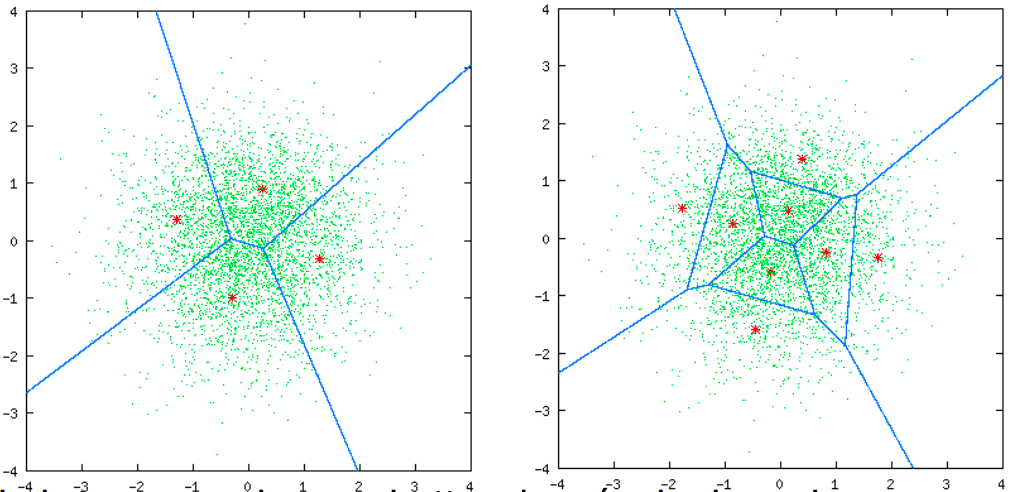
\includegraphics[width=0.6\textwidth]{images/rodzielania_2.png}
  \caption{Konstrukcja słownika metodą rozdzielania. Kolejne etapy konstrukcji wektorów kodowych
    (zaznaczone czerwonymi punktami) na zbiorze uczącym (zaznaczony kolorem zielonym). Źródło \cite{mwilczewski}.}
  \label{fig:rozdzielania_2}
\end{figure}

\subsection{Algorytmy budowy słownika}

\subsubsection{Algorytm popularności}

Algorytm popularności jest prostym algorytmem generacji książki kodowej. Opisuje się go w sposób następujący:

\begin{itemize}
  \item wektorami kodowymi staje się ustalona liczba wektorów danych najczęściej występujących
        w obrazie (konieczne jest ustalenie progu liczby wystąpień),
  \item algorytm wyróżnia się stosunkowo małą złożonością obliczeniową i prostotą implementacji,
  \item wadą podstawowej wersji algorytmu popularności jest wprowadzanie do książki kodowej podobnych wartości (dominujących).
        Redukcję rozmiaru książki uzyskać można przez usunięcie bliskich (w sensie przyjętej metryki) wektorów i 
        wprowadzenie kolejnych wektorów pod względem liczby wystąpień.
        
        \begin{figure}[H]
          \centering
          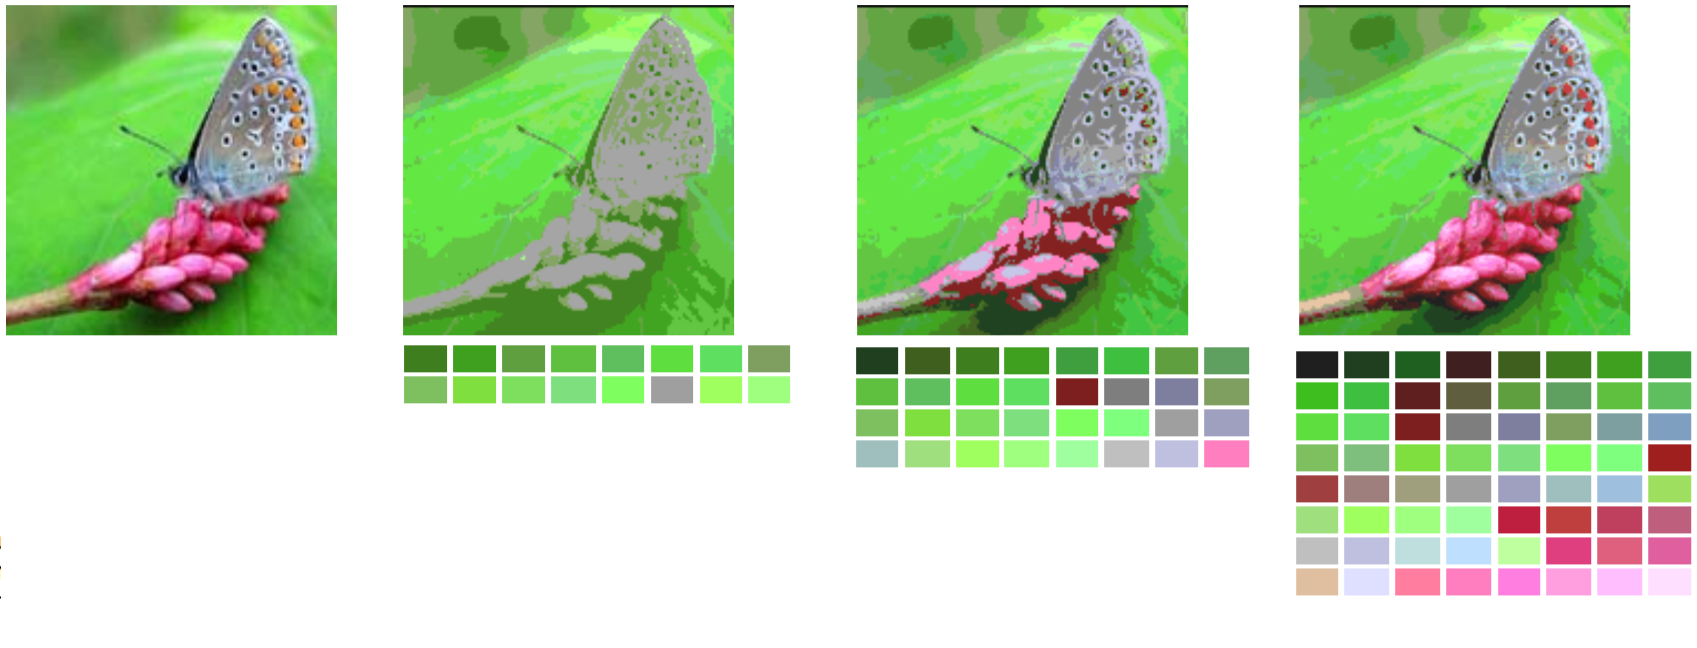
\includegraphics[width=0.6\textwidth]{images/motyle_2.png}
          \caption{Przykład kwantyzacji wektorowej przeprowadzonej z książką kodową skonstruowaną zgodnie z algorytmem popularności.
            Efekt kwantyzacji wektorowej z książkami kodowymi rozmiaru odpowiednio: 16, 32 oraz 64. Źródło \cite{aprzelaskowski}.}
          \label{fig:motyle_2}
        \end{figure}
        
\end{itemize}

\subsubsection{Algorytm Lindego-Buza-Graya}

Algorytm Lindego-Buza-Graya (LBG), powstał 1980, służy on do generowania książki kodowej \cite{lbg1980}. W celu wyznaczenia książki kodowej należy:

\begin{itemize} 
  \item określić wektory danych zbioru uczącego. Spośród wszystkich $N$ wektorów wejściowych
        wybrać losowo $K$ wektorów stanowiących wstępną wersję słownika,
  \item korzystając z metryki euklidesowej, $d(X,Y)$, dokonać klasteryzacji wektorów danych wokół słów kodowych bieżącej wersji słownika
        \begin{itemize}
          \item wybrać każdy kwadrat z obrazu o rozmiarze $(4 \times 4)$ i sprawdzić, któremu reprezentantowi ze słownika jest najbliżej do
                aktualnego kwadratu. Każdy piksel wewnątrz tego kwadratu należy porównać ze sobą i wyliczyć ich różnice w kwadracie.
                
                \begin{equation}
                  d(B_{m}, C_{i}) < d(B_{m}, C_{j})
                \end{equation}
                
                gdzie:
                \begin{itemize}[label=]
                  \item $B_{m}$ - blok obrazu,
                  \item $C_{i}$ - słowo kodowe ze słownika
                  \item $C_{j}$ - kolejne słowo kodowe ze słownika
                \end{itemize}
                
          \item następnie należy obliczyć sumę różnic 16 kwadratów
          \item sprawdzić kwadrat obrazu z każdym reprezentantem słownika
          \item przypisać wybrany kwadrat do reprezentanta słownika
        \end{itemize}
  \item wyznaczyć globalny błąd kwantyzacji popełniony w bieżącej iteracji czyli wykonujemy sumowanie wszystkich
        znalezionych odległości miedzy poszczególnymi kwadratami a centroidami z słownika
        
        \begin{equation}
          \label{eq:lbg_error}
          e = \sum_{i=1}^K \sum_{x\in\mathbb{R}} d(X, Y_{i}) 
        \end{equation}
        
  \item sprawdzić czy popełniany błąd zmienił się względem poprzedniej iteracji jeśli nie ma to kończymy algorytm
        (dla uproszczenia ustaliliśmy, że liczbę iteracji będzie podawana z ręki)
  \item wyznaczyć centroidy każdego regionu decyzyjnego i uczynić je wektorami kodowymi kolejnej iteracji słownika. Przejść do kroku 2.
\end{itemize}

Problemy tego algorytmu:

\begin{itemize}
  \item wrażliwość na inicjalną postać książki kodowej
  \item problem pustych przedziałów
\end{itemize}

\subsection{Miary podobieństwa obrazów}

\subsubsection{PSNR}

Szczytowy stosunek sygnału do szumu, (ang. \emph{peak signal-to-noise ratio (PSNR)}) – stosunek maksymalnej mocy sygnału do mocy szumu zakłócającego ten sygnał.  

Najczęściej PSNR stosowany jest do oceny jakości kodeków wykorzystujących stratną kompresję obrazków. 
W takim przypadku sygnałem są nieskompresowane dane źródłowe, a szumem – artefakty (zniekształcenia) spowodowane zastosowaniem kompresji stratnej. 

W celu wyznaczenie PSNR, należy najpierw obliczyć współczynnik MSE (błąd średniokwadratowy) bazując na obu porównywanych obrazkach za pomocą wzoru:

\begin{equation}
    \mathrm{MSE} = \frac{1}{n \cdot m} \sum_{i=1}^N \sum_{j=1}^M ([f(i, j) - f^{'}(i, j)])^2
\end{equation}

gdzie:
\begin{itemize}[label=]
  \item $n, m$ - wymiary obrazu w pikselach,
  \item $f(i, j)$ - wartość piksela o współrzędnych $(i, j)$ obrazu oryginalnego
  \item $f^{'}(i, j)$ - wartość piksela o współrzędnych $(i, j)$ obrazu poddanego kompresji i dekompresji
\end{itemize}

Następnie wyliczoną wartość MSE należy podstawić do końcowego wzoru: 

\begin{equation}
    \mathrm{PSNR} = 10 \cdot \log_{10} \frac{[\max(f(i,j))]^2}{MSE}
\end{equation}

gdzie:
\begin{itemize}[label=]
  \item $\max(f(i,j))$ - wartość maksymalna danego sygnału; w przypadku obrazów zwykle jest to wartość stała,
        np. dla obrazów monochromatycznych o reprezentacji 8-bitowej wynosi 255.
\end{itemize}

\subsubsection{SSIM}

Podobieństwo strukturalne miarą indeksu (ang. \emph{structural similarity index measure}) jest to metoda, która służy 
do pomiaru podobieństwa między dwoma obrazami. Indeks SSIM to pomiar jakości obrazu bazowego (nieskompresowanego) 
do obrazu po przekształceniach. SSIM to model oparty na percepcji, który traktuje degradację obrazu jako postrzeganą zmianę
w informacjach strukturalnych, przy jednoczesnym uwzględnieniu ważnych zjawisk percepcyjnych, w tym zarówno terminów maskowania 
luminancji, jak i maskowania kontrastu. Różnica w stosunku do innych technik, takich jak MSE lub PSNR,
polega na tym, że te podejścia szacują błędy bezwzględne. Idea informacji strukturalnych polega na tym, że piksele mają silne współzależności,
zwłaszcza gdy są znajdują się blisko siebie w przestrzenni. Zależności te niosą ważne informacje o strukturze obiektów \mbox{na scenie wizualnej \cite{channappayya2008rate}.}

Algorytm SSIM:

\begin{equation}
    \mathrm{SSIM}(x, y) = \frac{(2\mu_{x}\mu_{y} + c_{1}) \cdot (2\delta_{xy} + c_2)}{(\mu_{x}^2 + \mu_{y}^2 + c_{1}) \cdot (\delta_{x}^2 + \delta_{x}^2 + c_2)}
\end{equation}

gdzie:
\begin{itemize}[label=]
  \item $\mu_{x}$ - średnia x
  \item $\mu_{y}$ - średnia y
  \item $\delta_{x}^2$ - odchylenie od x
  \item $\delta_{y}^2$ - odchylenie od y
  \item $\delta_{xy}$ - kowariancja x i y
\end{itemize}

\subsubsection{FSIM}

Zastosowanie wskaźnika podobieństwa funkcji (ang. \emph{A Feature Similarity Index}) do oceny jakości obrazu, 
jest zagadnieniem skoncentrowanym wokół pomiaru podobieństwa między dwoma obrazami.
W celu interpretacji danego wskaźnika wymagane jest wyjaśnienie dwóch pojęć: zgodności fazowej (PC) oraz wielkości gradientu (GM) \cite{fsim_theory}.

\paragraph{Zgodność fazowa (ang. \emph{Phase Congruency}) (PC):}
Nową metodą wykrywania cech obrazu jest zgodność fazowa. Ważną cechą charakterystyczną zgodności fazowej jest to,
że jest stała dla zmiennych wartości światła na obrazie. Wskaźnik ten podkreśla cechy obrazu w częstotliwości fazowej. 
Jest to wartość niezmienna dla kontrastu. Na podstawie metody opisanej przez P. Kovesi, szeroko stosowanej w literaturze, 
można wyznaczyć wzór na obliczanie mapy zgodności fazowej dla obrazu \cite{pc}:

\begin{equation}
  PC(x) = \frac{|E(x)|}{(\varepsilon + \sum\limits{_{n}} A_n(x))}
\end{equation}

\paragraph{Wielkość gradientu  (ang. \emph{Gradient Magnitude}) (GM):}
Obliczanie gradientu obrazu jest bardzo tradycyjnym tematem w cyfrowym przetwarzaniu obrazu. 
Maski splotu są używane do wyrażania operatorów gradientu. Istnieje wiele masek konwolucyjnych do pomiaru gradientów. 
Jeśli $f(x)$ jest obrazem, a $Gx$ oraz $Gy$ to odpowiednio jego gradient poziomy i pionowy. 
Wtedy wielkośc gradientu $f(x)$ można zdefiniować następująco \cite{gm}:

\begin{equation}
  \sqrt{G^2_x+G^2_y}
\end{equation}

\paragraph{Algorytm FSIM \cite{fsim_alg}:}
Obliczanie indeksu FSIM składa się z dwóch etapów. 
W pierwszym etapie obliczana jest lokalna mapa wartości, a następnie w drugim etapie łączy się lokalne mapy podobieństwa w jeden wynik.
Wyliczany jest następnie oddzielny pomiar podobieństwa cech pomiędzy $f_1(x)$ i $f_2(x)$ obliczając wartości po dwie 
składowe na pomiar dla PC lub GM. Najpierw, miara podobieństwa dla $PC_1 (x)$ i $PC_2(x)$ jest zdefiniowana jako:

\begin{equation}
  S_{PC}(x) = \frac{2PC_1(x) \cdot PC_2(x) + T_1}{PC^2_1(x) + PC^2_2(x) + T_1}
\end{equation}

gdzie:
\begin{itemize}[label=]
  \item $T_1$ - dodatnia stała zwiększająca stabilność $S_PC$
\end{itemize}

Podobnie porównuje się wartości GM $G_1(x)$ i $G_2(x)$, a miarę podobieństwa definiuje się jako:

\begin{equation}
  S_G(x) = \frac{2G_1(x) \cdot G_2(x) + T_2}{G^2_1(x) + G^2_2(x) + T_2}
\end{equation}

gdzie:
\begin{itemize}[label=]
  \item $T_2$ - dodatnia stała zależna od dynamicznego zakresu wartości $GM$
\end{itemize}

Następnie $S_{PC}(x)$ i $S_G(x)$ są łączone, aby uzyskać podobieństwo $S_L(x)$ z $f_1(x)$ i $f_2(x)$. $S_L(x)$ jest definiowane jako:

\begin{equation}
  S_L(x) = [S_{PC}(x)]^\alpha \cdot [S_G(x)]^\beta
\end{equation}

gdzie:
\begin{itemize}[label=]
  \item $\alpha$, $\beta$ - parametry używane do dostosowania względnego znaczenia cech PC i GM
\end{itemize}

Po uzyskaniu podobieństwa $S_L(x)$ w każdym miejscu $x$ można obliczyć całkowite podobieństwo między $f_1$ i $f_2$. 
Jednak różne lokalizacje mają różny wpływ na postrzeganie obrazu przez HVS (ludzki system widzenia). 
Na przykład lokalizacje krawędzi przekazują ważniejsze informacje wizualne niż lokalizacje na gładkim obszarze. 
Ponieważ ludzka kora wzrokowa jest wrażliwa na struktury zgodne fazowo \cite{kora_wzrokowa}, wartość PC w danej 
lokalizacji może odzwierciedlać prawdopodobieństwo, że jest to dostrzegalnie istotny punkt obrazu. 
Intuicyjnie, dla danej lokalizacji $x$, jeśli którykolwiek wartość z $f_1(x)$ i $f_2(x)$ ma znaczącą wartość PC, 
oznacza to, że ta pozycja $x$ będzie miała duży wpływ na HVS w ocenie podobieństwa między $f_1$ i $f_2$. 
Dlatego używa się wartości maksymalnych $PC_m(x) = max (PC_1(x), PC_2(x))$, aby nadać wagę parametrowi $S_L(x)$ w 
ogólnym podobieństwie między $f_1$ i $f_2$, i odpowiednio zdefiniowano indeks FSIM między $f_1$ i $f_2$ w sposób przedstawiony poniżej:

\begin{equation}
  \mathrm{FSIM} = {{\sum\limits {_{{\bf x} \in \Omega } {S_{L}}({\bf x}) \cdot PC_{m}({\bf x})} } \over {\sum\limits {_{{\bf x} \in \Omega } PC_{m}({\bf x})}}}
\end{equation}

gdzie:
\begin{itemize}[label=]
  \item $\Omega$ - dziedzina przestrzeni obrazu
\end{itemize}

\subsubsection{RMSE}

Podstawowy błąd średniokwadratowy (RMSE) - jest to reguła, która mierzy średnią wielkość błędu. Jest to pierwiastek kwadratowy każdej różnicy między prognozowaną a odpowiadającą jej wartościom, podniesiona do kwadratu, a następnie uśredniona w próbie. Ponieważ błędy są podnoszone do kwadratu, zanim zostaną uśrednione, sprawia to, że RMSE nadaje stosunkowo dużą wagę dużym błędom. Oznacza to, że RMSE jest najbardziej przydatny, gdy duże błędy są szczególnie niepożądane \cite{rmse}.

Wzór RMSE:

\begin{equation}
    \mathrm{RMSE}=\sqrt{\frac{1}{n}\sum_{j=1}^{n}(y_j - \hat{y}_j)^2}
\end{equation}

gdzie:
\begin{itemize}[label=]
  \item $n$ - liczba prób,
  \item $y_{j}$ - prognozowana wartość błędu,
  \item $\hat{y_{j}}$ - rzeczywista wartość błędu \cite{rmse}.
\end{itemize}

\subsubsection{NRMSE}

Znormalizowany błąd średniokwadratowy (NRMSE) - ułatwiający porównywanie zestawów danych lub modeli o różnych skalach. Często wykorzystywanymi środkami normalizacji jest średnia lub zakres (zdefiniowany jako wartość maksymalna minus wartość minimalna mierzonych danych). NRMSE jest zazwyczaj wyrażana w procentach.

Wzór NRMSE:

\begin{equation}
    \mathrm{NRMSE} = \frac{\mathrm{RMSE}}{y_{max} - y_{min}}
\end{equation}

gdzie:
\begin{itemize}[label=]
  \item $\mathrm{RMSE}$ - Podstawowy błąd średniokwadratowy
  \item $y_{max}$ - wartość maksymalna
  \item $y_{min}$ - wartość minimalna
\end{itemize}

\subsection{Miary kompresji}

\subsubsection{CR}

Współczynnik kompresji danych (\textit{ang. data compression ratio}), znany również jako moc kompresji, jest miarą względnego zmniejszenia rozmiaru reprezentacji danych, który otrzymywany jest w procesie kompresji danych. Zwykle definiowany jest jako stosunek między rozmiarem nieskompresowanym a rozmiarem po kompresji:

\begin{equation}
    \mathrm{CR} = \frac{\mathrm{rozmiar\;przed\;kompresją}}{\mathrm{rozmiar\;po\;kompresji}}
  \label{eq:cr}
\end{equation}

Zatem w wyniku kompresji pliku o rozmiarze 10 MB do 2 MB, otrzymujemy współczynnik kompresji 10/2 = 5, często zapisywany jako wyraźny współczynnik, 5:1 \cite{compression_ratio}.

\subsubsection{BPP}

Średnia bitowa (ang. \emph{Bits Per Pixel}) (BPP) określa liczbę bitów przypadającą na 1 piksel zakodowanego obrazu. Początkowo każdy nasz plik miał 8 bitów na piksel. Stąd wzór ten dotyczy danego typu obrazów, które w naszym przypadku są 8-mio bitowe. Na przykład, jeśli stopień kompresji, który możemy obliczyć ze wzoru (\ref{eq:cr}) wynosi 4, daje nam średnią bitową wynoszącą 2 bity na piksel.

\begin{equation}
    \textrm{BPP} = \frac{8}{\textrm{CR}}
\end{equation}


\subsection{Kodowanie rożnicowe}
\label{sec:roznicowe}

Kodowanie różnicowe (ang. \emph{differential coding}) polega na porównaniu każdej ramki z ramką
poprzednią oraz kodowaniu tylko tych pikseli, których wartość zmienia się. W wyniku
zmniejszenia wartości, otrzymujemy mniej informacji do zakodowania. Jeśli kompresja ma
być bezstratna, to wówczas każda zmiana wartości piksela musi być uwzględniona. Algorytm może stać się wtedy nie efektywny pod względem czasu przetwarzania, jak również objętość sygnału po kompresji może przewyższać objętość tego samego sygnału przed kompresja.  Weźmy pod uwagę sygnały dwuwymiarowe, którymi są obrazy, możemy zaobserwować podobieństwo między sąsiednimi pikselami. Modelowanie danych wykonuje się w takim przypadku przez usunięcie jak największej ilości informacji wzajemnej, które występują między sąsiadującymi pikselami, jest to zatem pewien proces dekompozycji danych. Po tym etapie możemy uznać, iż przekształcony sygnał cyfrowy stanowi w przybliżeniu zbiór symboli wzajemnie niezależnych. Wówczas dla danych tego typu, entropię bezwarunkową może być wyznaczona ze wzoru:

\begin{equation}
    \label{eq:entropia}
    H = -\sum_{i=\varepsilon_{\textrm{min}}}^{e_{\textrm{emax}}} p_{i} \cdot \log_{2} p_{i}
\end{equation}

gdzie:
\begin{itemize}[label=]
 \item $p_i$ -- prawdopodobieństwo wystąpienia symbolu z alfabetu o indeksie i
\end{itemize}

Wynikiem jest entropia, która daje informacje o minimalnej średniej liczbie bitów potrzebnej do zakodowania jednego symbolu przy użyciu jednej z metod statycznego kodowania entropijnego (np. kodu Huffmana lub Golomba).

Algorytm kodowania różnicowego polega na kodowaniu różnic pomiędzy elementami. Ma to taką zaletę, że sygnał rzadko zmienia się gwałtownie, więc różnice pomiędzy sąsiednimi elementami są małe. Implementacja algorytmu działa w następujący sposób:

\begin{enumerate}
 \item Lewy górny piksel obrazu jest zapisywany do pliku wynikowego bez zmian, ponieważ nie posiada sąsiadów.
 \item Pozostałe piksele w każdym wierszu kodowane są różnicowo z wykorzystaniem lewego sąsiada $e = P(0) - P(1)$, a pozostałe piksele w pierwszej kolumnie z wykorzystaniem górnego sąsiada $e = P(0) - P(2)$. Numerację pikseli sąsiedztwa przedstawiono na rysunku \ref{fig:piksele_sasiedztwa}.
\end{enumerate}
To bardzo prosty algorytm do realizacji sprzętowego przetwarzania danych oraz w kodowaniu audio.

\begin{figure}[H]
  \centering
  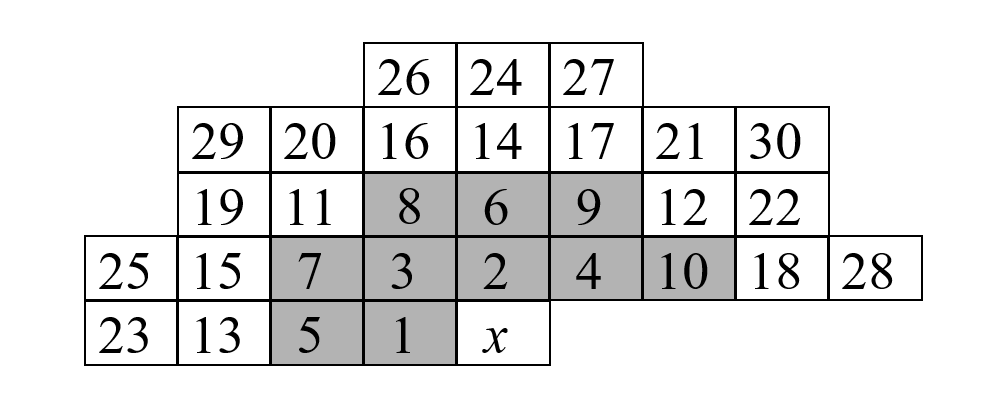
\includegraphics[width=0.6\textwidth]{images/piksele_sasiedztwa.png}
  \caption{Numeracja pikseli sąsiedztwa. Źródło \cite{differential_coding}.}
  \label{fig:piksele_sasiedztwa}
\end{figure}

Algorytm różnicowego kodowania średniej kodują różnice na podstawie średniej sąsiadów. Przebieg algorytmu możemy opisać w następujący sposób:
\begin{enumerate}
 \item pierwszy wiersz i pierwszą kolumnę kodujemy różnicowo,
 \item każdy piksel począwszy od drugiego wiersza i drugiej kolumny kodujemy średnią wartością (wymagana jest dostępność w dekoderze lewego sąsiada i dwóch sąsiednich pikseli z wiersza powyżej \cite{differential_coding}.
\end{enumerate}


Algorytmy metod adaptacyjnych są to zestaw trzech prostych predyktorów z przełączaniem kontekstowym. Konteksty wyznaczane są na podstawie trzech sąsiednich pikseli $P(1)$, $P(2)$, $P(3)$. Wartość przewidywana obliczana jest zgodnie z następującą zasadą:


\begin{equation}
\hat{x}_{\mathrm{MED}}=\left\{\begin{array}{l}
\min (P(1), P(2)) \text{ dla } P(3) \geq \max(P(1), P(2)) \\
\max (P(1), P(2)) \text{ dla } P(3) \leq \min(P(1), P(2))
\end{array}\right.
\end{equation}

oraz w pozostałych przypadkach: 


\begin{equation}
\hat{x}_{\mathrm{MED}}= \max(P(1) + P(2) - P(3))
\end{equation}

\subsection{Kodowanie Golomba}
\label{sec:golomb}

Kodowanie Golomba (ang. \emph{Golomb coding}) jest bezstratną metodą kompresji danych wykorzystująca rodzinę kodów kompresji danych wynalezionych przez Solomona W. Golomb w latach 60. Alfabety zgodne z rozkładem geometrycznym będą miały kod Golomba jako optymalny kod prefiksu, dzięki czemu kodowanie Golomba będzie wysoce odpowiednie w sytuacjach, w których wystąpienie małych wartości w strumieniu wejściowym jest znacznie bardziej prawdopodobne niż duże wartości.

Przed wykorzystaniem kodera Golomba zwrócono uwagę, na fakty związane z błędami predykcji powstałymi w etapie modelowania. Po pierwsze zakres wartości błędów predykcji $e(n)$ podwaja się w stosunku do zakresu próbek $x(n)$ kodowanego sygnału (np. dla próbek 8-bitowych błędy predykcji przyjmują wartości z przedziału od $-255$ do $255$). Jest ot zatem zakres 9-bitowy.

Ponadto, aby można było kodować te błędy predykcji przy użyciu kodu Golomba, niezbędna jest odpowiednia transformacja wartości $e(0)$ na liczby nieujemne.

Najprostszym podejściem jest algorytm zapisu wartości absolutnej błędu $e(0)=|e(0)|$, a następnie zapis bitu znaku, np. 1 odpowiada liczbie nieujemnej), o ile $e(0)>0$, w przypadku zera nie ma potrzeby zapisywać bit znaku do pliku wynikowego (dekoder zauważy, że nie ma zer ujemnych, więc nie wczyta bitu znaku).

Wynikowy zakres liczb $e(0)$ (nazywanych dalej zmodyfikowanymi błędami predykcji) jest przedział od $0$ do $2^8 - 1$, dzięki czemu możliwe jest ich kodowanie przy użyciu kodu Golomba.

\textbf{Algorytm działania kodera Golomba}

W pierwszym kroku wykonujemy konwersje liczby całkowitej $e(n)$ na parę liczb $u_G$ oraz $v_G$:
  
\begin{equation}
u_{G}=\left\lfloor\frac{\bar{e}(0)}{m}\right\rfloor
\end{equation}	
  
dla $m > 1$:
  
\begin{equation}
v_{G}=\bar{e}(0)-u_{G} \cdot m
\end{equation}	
  
Dla $m = 1$, wartość $v_G$ nie istnieje. Każda kodowana wartość $e(0)$ wymaga indywidualnej wartości parametru $m$, który wyliczamy ze wzoru:
  
\begin{equation}
m=\left[-\frac{\log_{10}(1+p)}{\log_{10} p}\right]
\end{equation}
  
gdzie:

$p$ - obliczamy wcześniej $S$ jako średnią zrzutowanych błędów predykcji w najbliższym otoczeniu:
  
\begin{equation}
S=\frac{1}{x} \sum_{j=1}^{3} \bar{e}(j)
\end{equation}
  
gdzie:
  
$x$ - liczba ilości sąsiednich pikseli, które możliwe jest od drugiego wiersza i drugiej kolumny. W przypadku pierwszego wiersza i pierwszej kolumny:

\begin{equation}
\begin{array}{l}
p=\frac{S-1}{S}, \text { dla } S \geq 2 \\
p=0,5 \text { dla } S<2
\end{array}
\end{equation}

Dopiero mając $p$ podstawiamy do wzoru na $m$. Liczba $m$ powinna być od $1$ do $2^8$.

Mając wyznaczoną wartość $e(0)$ oraz $m$, wyliczamy $u_G$ oraz $v_G$. Następnie wysyłamy liczbę $u_G$ w postaci kodu unarnego ($u_G$ zer zakończonych jedynką), a potem liczbę $v_G$ jako kod dwufazowy z parametrem $m$:

Liczba $v_G$ kodowana jest za pomocą kodu dwufazowego z parametrem $m$ (to wersja kodu Huffmana dla źródła o $m$ równo prawdopodobnych symbolach). Przyjęcie pomocniczego parametru $k = \log_2 m$ oznacza, że w każdej grupie pierwszych $l = 2_k - m$ wartości kodowanych jest za pomocą $k - 1$ bitów, a pozostałych $m-l$ jest kodowanych w postaci liczby $v + k^2 - m$ za pomocą k bitów \cite{golomb}.

\textbf{Algorytm kodera liczby $v_G$}

Wejście: Liczba $v_G$ (k bitów):

\begin{enumerate}
  \item Jeśli $v_G < 1$ to wyślij liczbę $v_G$ ($k-1$ najmłodszych bitów) na wyjście,
  \item W przeciwnym wypadku wysłać $v_G = v_G + 1$ ($k$ bitów - zapis pozycyjny liczby binarnej) na wyjście,
\end{enumerate}

\textbf{Algorytm dekodera liczby $v_G$}

Wejście: Wczytać $k - 1$ bitów do liczby $v_G$:

\begin{enumerate}
  \item Jeśli $v_G < 1$ to liczbę $v_G$ jest już zdekodowana,
  \item W przeciwnym wypadku wczytać z wyjścia jeden bit do liczby $q$, a następnie policzyć 
  \begin{equation}
  v_{G}:=2 \cdot v_{G}+q-l ; \text { (liczba } k \text { bitowa })
  \end{equation}
\end{enumerate}

\textbf{Algorytm działania dekodera Golomba}

\begin{enumerate}
  \item Wczytujemy i zliczamy (jako wartość u) zera aż trafimy na jedynkę
  \item Następnie zastosować algorytm dekodera liczby $v_G$
  \item Odtwarzamy z pary liczb $u_G$ i $v_G$ wartość:
  
  \begin{equation}
  \bar{e}(0)=u_{G} \cdot m+v_{G}
  \end{equation}
  
  a po zakończonych obliczeniach jeśli $e(0) > 0$ wczytujemy jeszcze bit znaku, żeby odtworzyć pierwotną liczbę $e(0)$.	
  
\end{enumerate}

\newpage

\section{Eksperymenty w zakresie zaimplementowanych algorytmów oraz całego procesu kompresji}

\subsection{Jaki procent stanowi dana rozdzielczość
  obrazu względem wielkości zdefiniowanego słownika?}
  
 Przeprowadzono statyczną analizę stosunku części książki kodowej do rozmiaru zakodowanego przy użyciu kwantyzacji wektorowej bez uwzględniania średnich. Wyniki przedstawiono w tabeli (\ref{tab:procentowa_analiza_slownika}).

\begin{table}[!h]
  \caption{Procentowa analiza zależności części nagłówkowej względem wielkości obrazu oryginalnego oraz względem obrazu zakodowanego}\
  \label{tab:procentowa_analiza_slownika}
  \centering
  \begin{tabular}{cclclcl}
    \toprule
    \multirow{2}{*}{\begin{tabular}[c]{@{}c@{}} Rozdzielczość \\obrazu \end{tabular}} & \multicolumn{2}{c}{$C_S = 2^8$}                           & \multicolumn{2}{c}{$C_S = 2^9$}                           & \multicolumn{2}{c}{$C_S = 2^{10}$}                         \\
                   & $\frac{C_S}{I_S}$ & \multicolumn{1}{c}{$\frac{C_S}{Q_S}$} & $\frac{C_S}{I_S}$ & \multicolumn{1}{c}{$\frac{C_S}{Q_S}$} & $\frac{C_S}{I_S}$ & \multicolumn{1}{c}{$\frac{C_S}{Q_S}$} \\ 
    \midrule \\
    256 x 256 px   & 6.25\%            & 50.00\%                               & 12.50\%           & 64.00\%                               & 25.00\%           & 76.19\%                               \\
    512 x 512 px   & 1.56\%            & 20.00\%                               & 3.13\%            & 30.77\%                               & 6.25\%            & 44.44\%                               \\
    720 x 576 px   & 0.99\%            & 13.65\%                               & 1.98\%            & 21.93\%                               & 3.95\%            & 33.58\%                               \\
    1920 x 1080 px & 0.20\%            & 3.06\%                                & 0.40\%            & 5.32\%                                & 0.79\%            & 9.18\%                                \\
    3840 x 2160 px & 0.05\%            & 0.78\%                                & 0.10\%            & 1.39\%                                & 0.20\%            & 2.47\%                                \\
    \bottomrule
  \end{tabular}
\end{table}

Oznaczenia wykorzystane w tabeli:
\begin{itemize}[label=]
  \item $C_S$ - codebook size - rozmiar książki kodowej w bitach. Obliczany ze wzoru (\ref{eq:lgb_dict_size}).
  \item $I_S$ - image size - rozmiar obrazu oryginalnego.
  \item $Q_S$ - quantized size - rozmiar obrazu po klasycznej kwantyzacji wektorowej bez uwzględniania średnich z bloków (wielkość słownika + kodowanie poszczególnych bloków). Obliczany ze wzoru (\ref{eq:lgb_image_size}).
\end{itemize}

Tabela \ref{tab:procentowa_analiza_slownika} została sporządzona dla stałej wielkości bloku o rozmiarze 4 x 4 px.

\subsection{Algorytm LBG z losową inicjalizacją słownika}
\label{sec:lbg_psnr}

W kolejnym eksperymencie przebadano algorytm budowy słownika LBG. Przeprowadzono kwantyzację wektorową na blokach o rozmiarach $4 \times 4$ oraz dla książki
kodowej o długości $512$ elementów. Dane zebrano w \mbox{tabeli \ref{tab:lbg_random}} i podsumowano w tabeli \mbox{\ref{tab:lbg_summary}}.

\begin{table}[H]
  \caption{Porównanie jakości kwantyzacji algorytmu budowy słownika LBG z losową inicjalizacją słownika dla bloku $4 \times 4$ oraz długości słownika $512$.}
  \label{tab:lbg_random}
  \centering
  \begin{tabular}{@{}lrrrr@{}}
    \toprule
    Obraz              & PSNR {[}dB{]} & SSIM     & MSE        & NRMSE    \\ \midrule
    Aerial.bmp         & 30.308975     & 0.738150 & 269.074234 & 0.088749 \\
    airfield.bmp       & 29.847609     & 0.621790 & 305.594254 & 0.112432 \\
    airplane.bmp       & 32.766159     & 0.835739 & 112.650368 & 0.057495 \\
    baboonTMW.bmp      & 29.225130     & 0.619144 & 388.316032 & 0.145004 \\
    balloon.bmp        & 35.504876     & 0.879501 & 31.181279  & 0.050065 \\
    balloon\_noise.bmp & 35.510646     & 0.879980 & 31.957593  & 0.050894 \\
    BARB.bmp           & 30.544723     & 0.719523 & 220.033929 & 0.123536 \\
    BARB2.bmp          & 30.739427     & 0.753790 & 199.587676 & 0.112621 \\
    barb512.bmp        & 30.336805     & 0.699047 & 237.749905 & 0.119092 \\
    BOARD.bmp          & 33.838988     & 0.850642 & 74.120845  & 0.073532 \\
    boat512.bmp        & 31.022867     & 0.725675 & 150.630928 & 0.089032 \\
    boats.bmp          & 32.266624     & 0.809828 & 99.350383  & 0.076842 \\
    bridge.bmp         & 29.309403     & 0.638427 & 294.446346 & 0.135884 \\
    bridge256.bmp      & 29.204719     & 0.638050 & 320.350159 & 0.142547 \\
    camera256.bmp      & 32.096795     & 0.775423 & 238.143219 & 0.115080 \\
    couple.bmp         & 30.728604     & 0.709376 & 164.932125 & 0.099725 \\
    couple256.bmp      & 32.855874     & 0.824001 & 78.755783  & 0.194422 \\
    crowd512.bmp       & 31.652136     & 0.815185 & 144.212181 & 0.121814 \\
    EARTH.bmp          & 31.889207     & 0.813266 & 180.529541 & 0.139229 \\
    elaine.bmp         & 31.524373     & 0.705601 & 79.712097  & 0.062034 \\
    ELIF.bmp           & 34.798653     & 0.888926 & 47.819733  & 0.092001 \\
    finger.bmp         & 28.976954     & 0.782924 & 287.981743 & 0.136837 \\
    FROG512.BMP        & 29.215023     & 0.528005 & 277.108448 & 0.129976 \\
    GIRL.bmp           & 32.154535     & 0.801970 & 75.534510  & 0.061551 \\
    GOLD.bmp           & 31.309143     & 0.729300 & 101.270226 & 0.088009 \\
    GOLDHILL.BMP       & 31.057375     & 0.728247 & 108.036793 & 0.084831 \\
    harbour512.bmp     & 31.093608     & 0.714235 & 240.901379 & 0.117528 \\
    HOTEL.bmp          & 31.435559     & 0.783956 & 165.572328 & 0.118273 \\
    lax512.bmp         & 30.189473     & 0.618931 & 270.259842 & 0.184256 \\
    lenaTMW.bmp        & 31.481890     & 0.747129 & 118.296848 & 0.096867 \\
    lennagrey.bmp      & 32.377624     & 0.794924 & 91.050716  & 0.071973 \\
    man512.bmp         & 31.392019     & 0.740788 & 131.757545 & 0.094573 \\
    noisesquare.bmp    & 30.757530     & 0.629793 & 65.570068  & 0.042190 \\
    OMAHA.bmp          & 28.794700     & 0.652411 & 706.925873 & 0.153396 \\
    peppersTMW.bmp     & 31.985593     & 0.760791 & 98.846947  & 0.075693 \\
    SAILBOAT.bmp       & 31.483250     & 0.767148 & 134.057770 & 0.085355 \\
    seismic.bmp        & 35.929998     & 0.923327 & 19.705395  & 0.034543 \\
    SENA.bmp           & 33.949226     & 0.857894 & 52.210876  & 0.080610 \\
    SENSIN.bmp         & 31.768706     & 0.832904 & 82.924622  & 0.084624 \\
    shapes.bmp         & 34.324357     & 0.861644 & 71.168495  & 0.095598 \\
    SINAN.bmp          & 32.519610     & 0.829939 & 66.397598  & 0.062148 \\
    Tank512.bmp        & 32.088375     & 0.738335 & 66.664444  & 0.060426 \\
    Truck512.bmp       & 32.243722     & 0.779603 & 65.496967  & 0.073253 \\
    woman1.bmp         & 31.658150     & 0.741796 & 130.824505 & 0.080795 \\
    woman2.bmp         & 34.390173     & 0.863615 & 38.900913  & 0.050211 \\
    ZELDA.bmp          & 33.747423     & 0.828049 & 44.793265  & 0.057213 \\
    \bottomrule
  \end{tabular}
\end{table}


\begin{table}[H]
  \caption{Przedstawienie wartości minimalnej, maksymalnej oraz uśrednienie wyników dla poszczególnych metryk dla algorytmu LBG.}
  \label{tab:lbg_summary}
  \centering
  \begin{tabular}{@{}lrrrr@{}}
    \toprule
             & PSNR {[}dB{]} & SSIM     & MSE        & NRMSE    \\ \midrule
    Minimum  & 28.794700     & 0.528005 & 19.705395  & 0.034543 \\
    Maksimum & 35.929998     & 0.923327 & 706.925873 & 0.194422 \\
    Średnia  & 31.789057     & 0.760407 & 156.117538 & 0.096147 \\
    \bottomrule
  \end{tabular}
\end{table}

\FloatBarrier

\subsubsection{Wyznaczenie optymalnej liczby iteracji w algorytmie budowy słownika LBG}

Przeprowadzono kwantyzację dla każdego obrazu wymuszając wykonanie wszystkich $50$ iteracji. Dla każdej iteracji raportowano błąd obliczany zgodnie ze wzorem (\ref{eq:lbg_error}). Wyniki zbiorcze przedstawiono na rysunku \ref{fig:lbg_iterations}. Średni błąd dla każdej iteracji przedstawiono na rysunku \ref{fig:lbg_iterations_mean}.

\begin{figure}[H]
  \centering
  \centering
  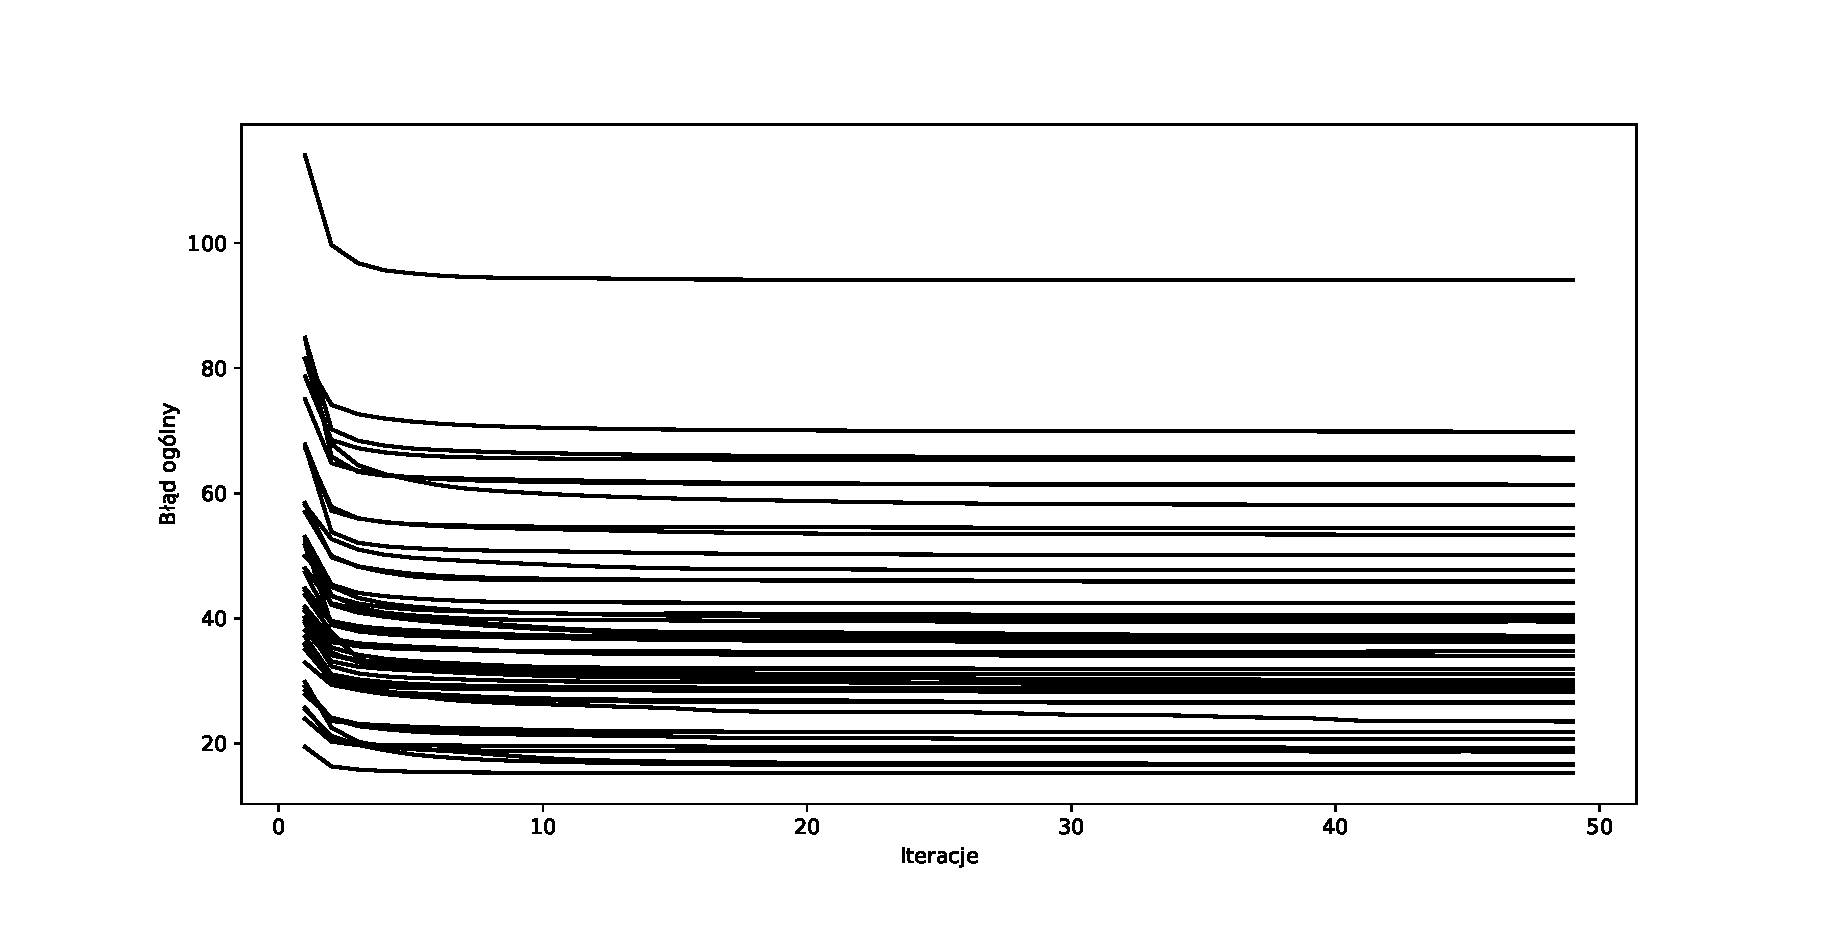
\includegraphics[width=.9\linewidth]{images/lbg_4x4_32_50_iterations.eps}
  \caption{Błędy w poszczególnych iteracjach algorytmu LGB dla wektorów 16 elementowych i słownikiem o długości 512.}
  \label{fig:lbg_iterations}
\end{figure}

\begin{figure}[H]
  \centering
  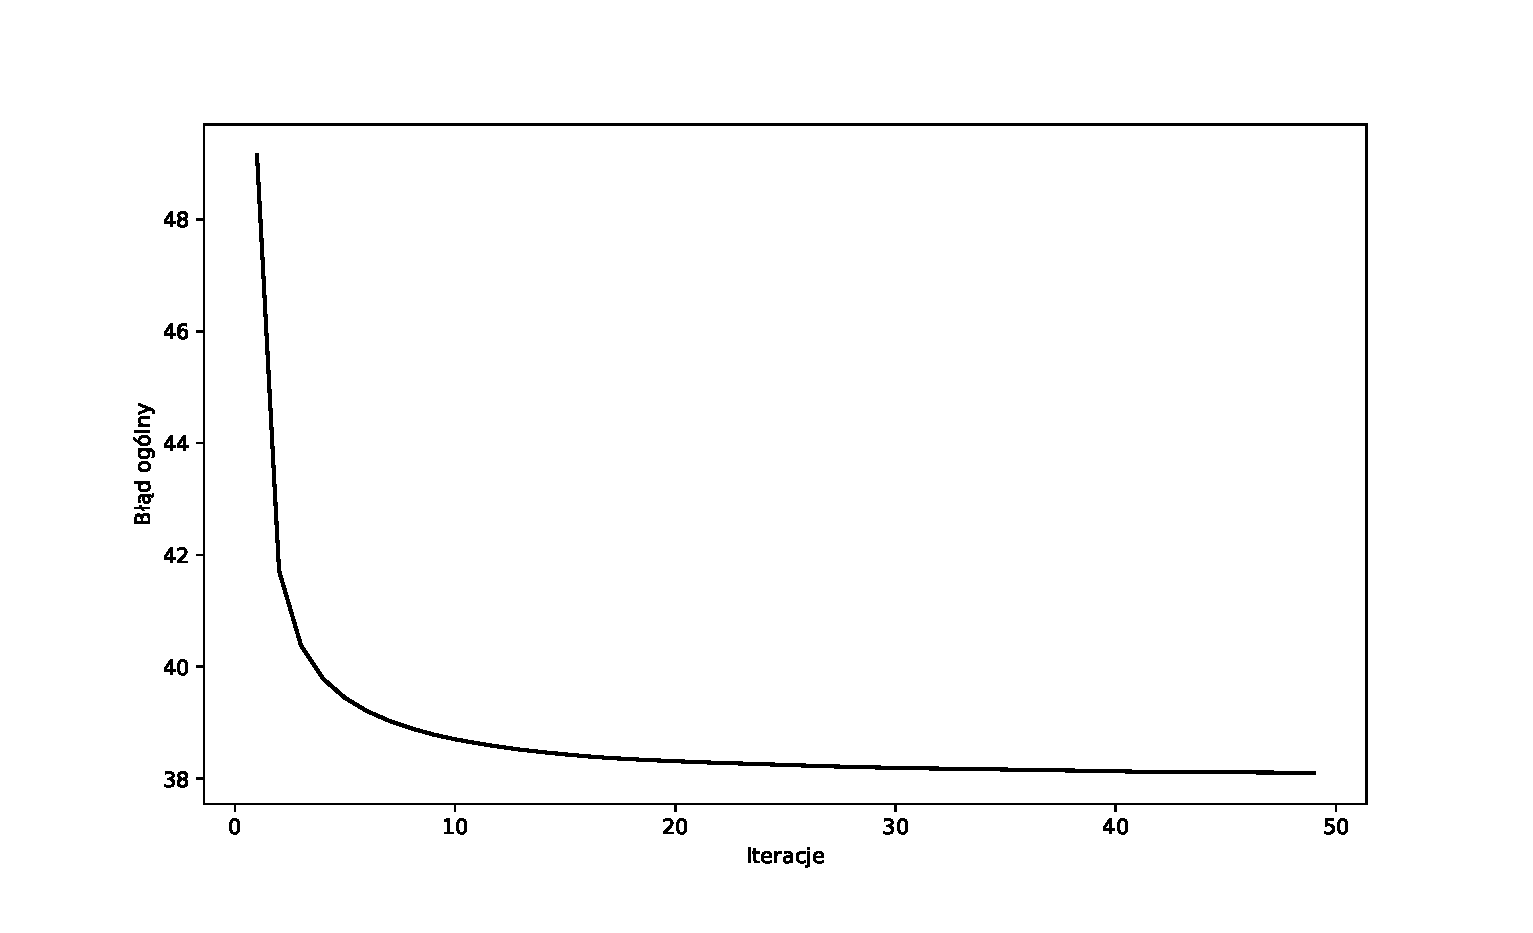
\includegraphics[width=.9\linewidth]{images/lbg_4x4_32_mean_iterations.eps}
  \caption{Średni błąd w poszczególnych iteracjach algorytm LGB dla wektorów 16 elementowych i słownikiem o długości 512.}
  \label{fig:lbg_iterations_mean}
\end{figure}

\subsection{Algorytm MRVQ z losową inicjalizacją słownika}

Przeprowadzono badanie algorytmu MRVQ z losowym słownikiem. Kwantyzację przeprowadzono na blokach o rozmiarach $4 \times 4$ oraz dla książki
kodowej o długości $512$ elementów. Dane zebrano w \mbox{tabeli \ref{tab:mrvq_random}} i podsumowano w tabeli \mbox{\ref{tab:mrvq_summary}}.

Uzyskane wyniki są podobieństwa obrazów są lepsze w porównaniu do wyników klasycznej kwantyzacji wektorowej zebranych w sekcji \ref{sec:lbg_psnr}. Średni poziom PSNR dla MRVQ wynosi 33.664910 [dB] a dla klasycznej kwantyzacji wektorowej wynosi 31.789057 [dB]. Oczywiście zysk jakości uzyskano dzięki stracie współczynnika kompresji wynikające z potrzeby przechowywania wartości średnich dla każdego bloku.

\begin{table}[h]
  \caption{Przedstawienie wartości minimalnej, maksymalnej oraz uśrednienie wyników dla poszczególnych metryk dla algorytmu MRVQ.}
  \label{tab:mrvq_summary}
  \centering
  \begin{tabular}{@{}lrrrr@{}}
    \toprule
             & PSNR {[}dB{]} & SSIM     & MSE        & NRMSE    \\ \midrule
    Minimum  & 29.379325     & 0.661741 & 8.685005   & 0.022933 \\
    Maksimum & 39.609384     & 0.967245 & 673.800110 & 0.388628 \\
    Średnia  & 33.664910     & 0.859542 & 142.266146 & 0.090000 \\
    \bottomrule
  \end{tabular}
\end{table}

\begin{table}[h]
  \caption{Porównanie jakości kwantyzacji algorytmu MRVQ z losową inicjalizacją słownika dla bloku $4 \times 4$ oraz długości słownika $512$.}
  \label{tab:mrvq_random}
  \centering
  \begin{tabular}{@{}lrrrr@{}}

    \toprule
    Obraz              & PSNR [dB] & SSIM     & MSE        & NRMSE    \\
    \midrule
    Aerial.bmp         & 31.325414 & 0.838639 & 206.558186 & 0.077759 \\
    airfield.bmp       & 30.840608 & 0.733311 & 616.739300 & 0.159723 \\
    airplane.bmp       & 34.493424 & 0.916806 & 59.944592  & 0.041941 \\
    baboonTMW.bmp      & 29.837549 & 0.740805 & 302.010212 & 0.127878 \\
    balloon.bmp        & 39.502431 & 0.959524 & 31.986904  & 0.050708 \\
    balloon\_noise.bmp & 39.609384 & 0.958425 & 12.200263  & 0.031446 \\
    BARB.bmp           & 31.996066 & 0.858178 & 123.859623 & 0.092686 \\
    BARB2.bmp          & 31.954561 & 0.864515 & 120.047174 & 0.087343 \\
    barb512.bmp        & 31.859472 & 0.850585 & 129.981781 & 0.088057 \\
    BOARD.bmp          & 36.170801 & 0.920150 & 83.243762  & 0.077926 \\
    boat512.bmp        & 32.681597 & 0.848437 & 88.513115  & 0.068249 \\
    boats.bmp          & 34.282138 & 0.907079 & 53.116669  & 0.056186 \\
    bridge.bmp         & 30.424395 & 0.780987 & 289.719372 & 0.134789 \\
    bridge256.bmp      & 30.044354 & 0.773070 & 352.649445 & 0.149561 \\
    camera256.bmp      & 33.169167 & 0.841805 & 302.633728 & 0.129730 \\
    couple.bmp         & 32.546104 & 0.854006 & 116.577576 & 0.083842 \\
    couple256.bmp      & 34.703286 & 0.845815 & 314.672928 & 0.388628 \\
    crowd512.bmp       & 33.385017 & 0.899106 & 136.984058 & 0.118722 \\
    EARTH.bmp          & 32.826552 & 0.864470 & 296.390259 & 0.178397 \\
    elaine.bmp         & 33.287508 & 0.833254 & 45.968887  & 0.047108 \\
    ELIF.bmp           & 37.148792 & 0.949756 & 21.990341  & 0.062389 \\
    finger.bmp         & 29.726525 & 0.878141 & 157.704418 & 0.101261 \\
    FROG512.BMP        & 29.711200 & 0.661741 & 412.729481 & 0.158624 \\
    GIRL.bmp           & 35.259907 & 0.916269 & 32.797847  & 0.040559 \\
    GOLD.bmp           & 33.433986 & 0.864741 & 51.049732  & 0.062486 \\
    GOLDHILL.BMP       & 32.902191 & 0.854297 & 59.053673  & 0.062718 \\
    harbour512.bmp     & 32.128791 & 0.829542 & 158.326237 & 0.095280 \\
    HOTEL.bmp          & 33.205348 & 0.884421 & 103.708697 & 0.093605 \\
    lax512.bmp         & 30.733882 & 0.720240 & 199.029411 & 0.158121 \\
    lenaTMW.bmp        & 33.640265 & 0.860569 & 86.785583  & 0.082969 \\
    lennagrey.bmp      & 34.630062 & 0.898839 & 46.313889  & 0.051331 \\
    man512.bmp         & 33.057586 & 0.863485 & 75.862572  & 0.071762 \\
    noisesquare.bmp    & 31.067677 & 0.671197 & 58.469727  & 0.039840 \\
    OMAHA.bmp          & 29.379325 & 0.723564 & 673.800110 & 0.149759 \\
    peppersTMW.bmp     & 34.265375 & 0.867596 & 93.769455  & 0.073723 \\
    SAILBOAT.bmp       & 32.748110 & 0.858763 & 106.028950 & 0.075909 \\
    seismic.bmp        & 39.325434 & 0.967245 & 8.685005   & 0.022933 \\
    SENA.bmp           & 36.786062 & 0.941536 & 27.621506  & 0.058632 \\
    SENSIN.bmp         & 34.983614 & 0.941753 & 32.745911  & 0.053178 \\
    shapes.bmp         & 37.768621 & 0.936599 & 81.161709  & 0.102089 \\
    SINAN.bmp          & 36.004230 & 0.943409 & 30.180923  & 0.041901 \\
    Tank512.bmp        & 33.414859 & 0.832489 & 41.127480  & 0.047462 \\
    Truck512.bmp       & 33.791077 & 0.870388 & 37.876549  & 0.055706 \\
    woman1.bmp         & 33.235523 & 0.839538 & 212.144783 & 0.102886 \\
    woman2.bmp         & 38.422679 & 0.948926 & 22.523846  & 0.038207 \\
    ZELDA.bmp          & 36.874902 & 0.924915 & 28.957053  & 0.046001 \\
    \bottomrule

  \end{tabular}
\end{table}




\FloatBarrier

\subsection{Kodowanie różnicowe}

Zaimplementowano trzy metody kodowania różnicowego, których opisy przedstawiono w sekcji \ref{sec:roznicowe}.
Sporządzono wykres częstości występowania wartości (histogram) dla wartości wejściowych oraz wartości wyjściowych
z różnych metod kodowania różnicowego.

Na rysunku (\ref{fig:de_histogram_image}) porównanie rozkładów dla obrazu Lennagrey (linia niebieska) oraz różnicowego (linia czerwona).
Na podstawie rozkładów można wywnioskować, że wartości po kodowaniu różnicowym lepiej będą podlegać kompresji.
Przyjmuje się bowiem, że im bardziej niezrównoważone są wartości poszczególnych prawdopodobieństw (duża dysproporcja między prawdopodobieństwami najczęściej i najrzadziej występującymi), tym lepszą efektywność kodowania można uzyskać \cite{ulacha_roznicowe}.


\begin{figure}[H]
  \centering
  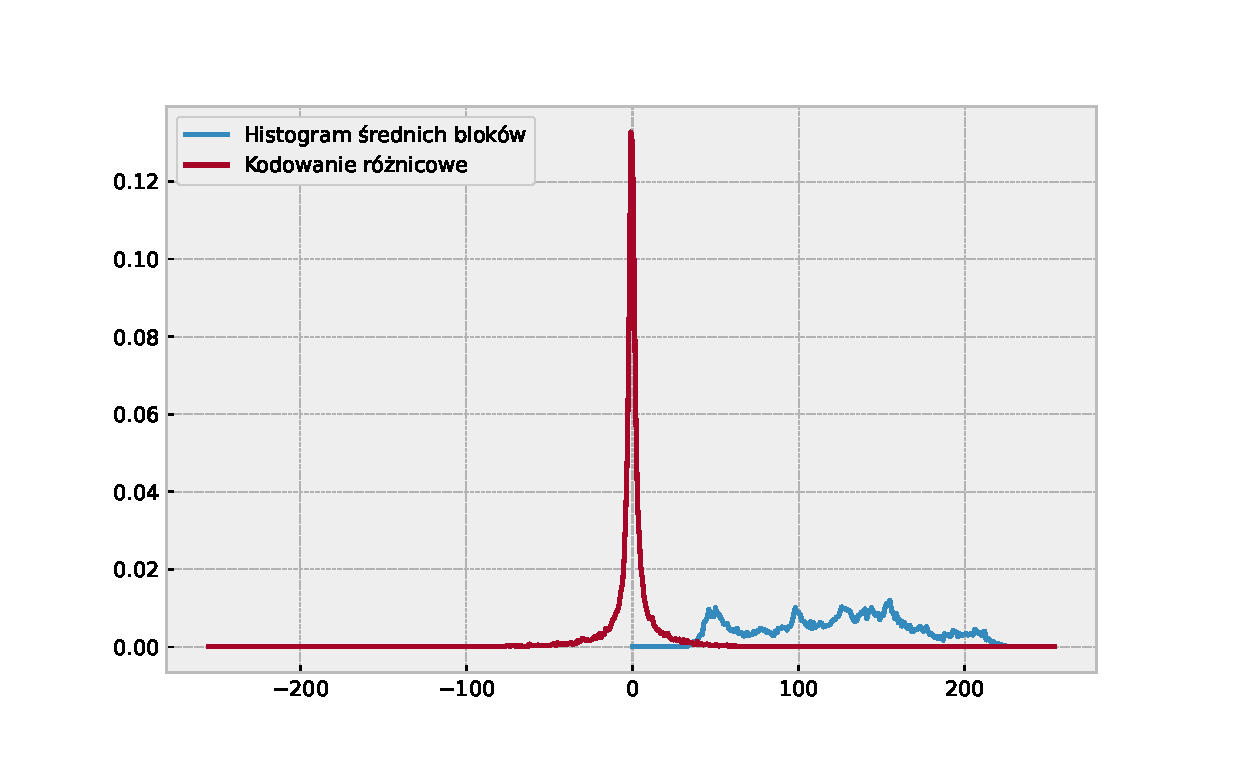
\includegraphics[width=.5\linewidth]{images/differential_encoding_histogram_image.eps}
  \caption{Porównanie histogramu wartości średnich bloków $4\times4$ obrazu \emph{lennagrey} i histogramu po kodowaniu różnicowym}
  \label{fig:de_histogram_image}
\end{figure}

\begin{figure}[H]
\begin{subfigure}{.49\textwidth}
  \centering
  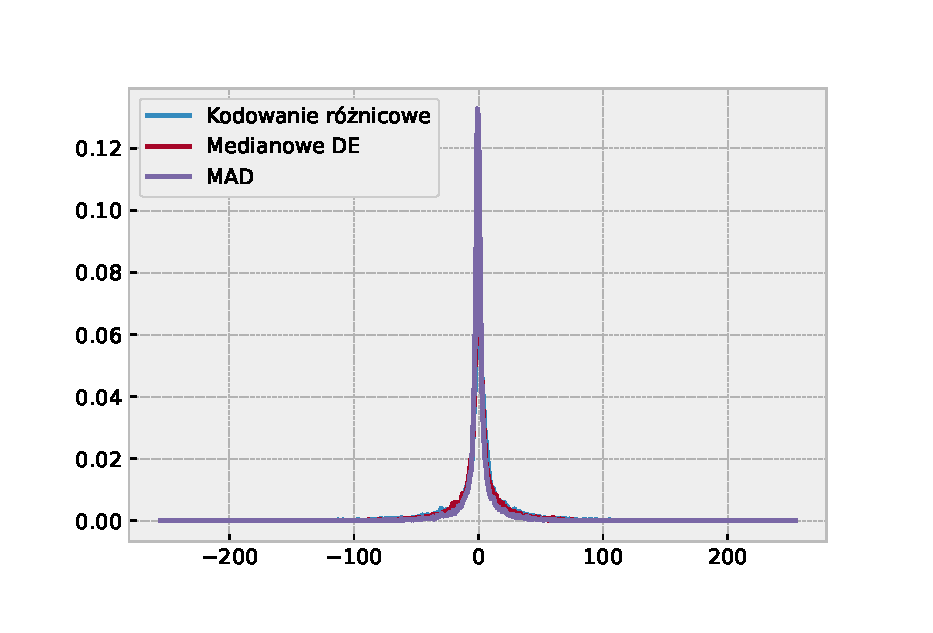
\includegraphics[width=.9\linewidth]{images/differential_encoding_histograms_comparison.eps}
  \caption{Porównanie histogramów dla metod kodowania różnicowego dla średnich z bloków $4\times4$ obrazu \emph{lennagrey}. Kolorem niebieskim oznaczono klasyczne kodowanie różnicowe, kolorem czerwonym oznaczono średnie kodowanie różnicowe, kolorem fioletowym adaptacyjny predyktor medianowy.}
  \label{fig:de_histograms_comparison}
\end{subfigure}
\begin{subfigure}{.49\textwidth}
  \centering
  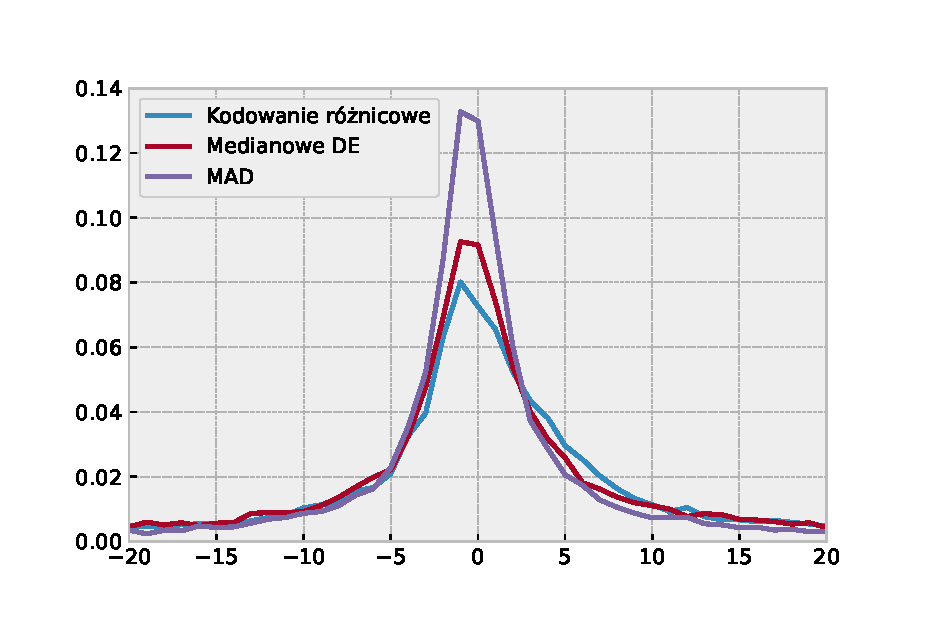
\includegraphics[width=.9\linewidth]{images/differential_encoding_histograms_comparison_zoom.eps}
  \caption{Porównanie histogramów dla metod kodowania różnicowego dla średnich z bloków $4\times4$ obrazu \emph{lennagrey}. Kolorem niebieskim oznaczono klasyczne kodowanie różnicowe, kolorem czerwonym oznaczono średnie kodowanie różnicowe, kolorem fioletowym adaptacyjny predyktor medianowy.}
  \label{fig:de_histograms_comparison_zoom}
\end{subfigure}
\end{figure}

% TODO: podmienić te obrazki aby nie było legendy


Przeprowadzono kodowanie wartości średnich z bloków uzyskiwanych w procesie kwantyzacji wektorowej z usuniętą średnią (MRVQ). Przeprowadzono porównanie trzech metod kodowania na podstawie pomiaru entropii według wzoru (\ref{eq:entropia}) w celu wybrania docelowej metody kodowania w całym procesie kompresji obrazów.

Do kodowania użyto trzech metod: kodowania różnicowego, średniego kodowania różnicowego i adaptacyjnego predyktora medianowego, które zostały opisane w sekcji \ref{sec:roznicowe}.

Uzyskane wyniki przedstawiono w tabeli (\ref{tab:differential_encoding_all}) oraz podsumowanie w tabeli (\ref{tab:differential_encoding_summary}). Najmniejsze wartości entropii uzyskuje adaptacyjny predyktor medianowy.
Z tego powodu używamy tej metody w procesie kompresji.

\begin{table}[H]
  \caption{Obliczenie entropii dla średnich uzyskanych w procesie MRVQ i kodowania tych średnich za pomocą kodowania różnicowego}
  \label{tab:differential_encoding_all}
  \centering
\begin{adjustbox}{center}
  \begin{tabular}{lrrrr}
    \toprule
    {}                 & \multicolumn{4}{c}{Entropia} \\
    \cmidrule(lr){2-5}
    {Obraz}            & \multicolumn{1}{c}{Wartości} & \multicolumn{1}{c}{Kodowania} & \multicolumn{1}{c}{Średniego kodowania}  & \multicolumn{1}{c}{Adaptacyjnego} \\
    {}                 & \multicolumn{1}{c}{wejściowych} & \multicolumn{1}{c}{różnicowego}        & \multicolumn{1}{c}{różnicowego} & \multicolumn{1}{c}{predyktora medianowego} \\
    \midrule
    Aerial.bmp         & 6.799397                     & 6.370003                               & 6.346111                                  & 6.281835                                   \\
    airfield.bmp       & 7.600676                     & 6.335829                               & 6.200263                                  & 6.115437                                   \\
    airplane.bmp       & 6.725235                     & 5.192151                               & 5.384822                                  & 4.951908                                   \\
    baboonTMW.bmp      & 7.133698                     & 6.231330                               & 6.065259                                  & 6.049762                                   \\
    balloon.bmp        & 7.305988                     & 4.676627                               & 4.567023                                  & 3.750564                                   \\
    balloon\_noise.bmp & 7.312372                     & 4.684539                               & 4.569674                                  & 3.760032                                   \\
    BARB.bmp           & 7.460040                     & 6.003715                               & 5.863538                                  & 5.321274                                   \\
    BARB2.bmp          & 7.389961                     & 5.914602                               & 5.700214                                  & 5.371247                                   \\
    barb512.bmp        & 7.551742                     & 5.994919                               & 5.846057                                  & 5.308187                                   \\
    BOARD.bmp          & 6.751369                     & 4.478934                               & 4.893147                                  & 3.820169                                   \\
    boat512.bmp        & 7.105094                     & 5.628897                               & 5.799380                                  & 5.270987                                   \\
    boats.bmp          & 7.039440                     & 5.171864                               & 5.334069                                  & 4.660202                                   \\
    bridge.bmp         & 7.612662                     & 6.195047                               & 6.272714                                  & 5.950704                                   \\
    bridge256.bmp      & 7.512977                     & 6.214165                               & 6.392970                                  & 5.996127                                   \\
    camera256.bmp      & 6.973989                     & 5.151811                               & 5.224229                                  & 4.781324                                   \\
    couple.bmp         & 7.337503                     & 5.876122                               & 5.893505                                  & 5.109491                                   \\
    couple256.bmp      & 6.343808                     & 5.386308                               & 5.370506                                  & 4.615757                                   \\
    crowd512.bmp       & 6.968875                     & 6.200433                               & 6.134625                                  & 5.794663                                   \\
    EARTH.bmp          & 5.252131                     & 4.741143                               & 4.695157                                  & 4.578020                                   \\
    elaine.bmp         & 7.455792                     & 5.606359                               & 5.410394                                  & 5.033493                                   \\
    ELIF.bmp           & 6.102673                     & 4.744612                               & 4.947915                                  & 4.425198                                   \\
    finger.bmp         & 7.167870                     & 6.845691                               & 6.611423                                  & 6.784109                                   \\
    FROG512.BMP        & 6.948923                     & 5.869151                               & 5.806952                                  & 5.749067                                   \\
    GIRL.bmp           & 7.211853                     & 5.725185                               & 5.554541                                  & 5.203274                                   \\
    GOLD.bmp           & 7.502927                     & 5.421554                               & 5.520399                                  & 4.952832                                   \\
    GOLDHILL.BMP       & 7.407802                     & 5.566452                               & 5.656368                                  & 5.139234                                   \\
    harbour512.bmp     & 6.539697                     & 5.021141                               & 5.401220                                  & 4.843480                                   \\
    HOTEL.bmp          & 7.492570                     & 5.644325                               & 5.707400                                  & 5.085551                                   \\
    lax512.bmp         & 6.638618                     & 5.944674                               & 5.753942                                  & 5.462067                                   \\
    lenaTMW.bmp        & 7.530290                     & 5.973761                               & 5.695504                                  & 5.131158                                   \\
    lennagrey.bmp      & 7.391431                     & 5.813837                               & 5.541977                                  & 4.937865                                   \\
    man512.bmp         & 7.248159                     & 5.948017                               & 5.806439                                  & 5.491626                                   \\
    noisesquare.bmp    & 4.114868                     & 3.967057                               & 3.874582                                  & 3.818463                                   \\
    OMAHA.bmp          & 7.438018                     & 7.141744                               & 6.895302                                  & 6.848980                                   \\
    peppersTMW.bmp     & 7.550972                     & 5.663923                               & 5.557934                                  & 4.959506                                   \\
    SAILBOAT.bmp       & 7.239532                     & 5.780576                               & 5.727559                                  & 5.380788                                   \\
    seismic.bmp        & 5.182019                     & 3.784849                               & 5.208382                                  & 4.175657                                   \\
    SENA.bmp           & 6.750098                     & 4.797344                               & 5.042326                                  & 4.371430                                   \\
    SENSIN.bmp         & 7.233915                     & 5.917481                               & 5.998098                                  & 5.571654                                   \\
    shapes.bmp         & 6.922706                     & 4.406802                               & 4.872293                                  & 3.495424                                   \\
    SINAN.bmp          & 7.265768                     & 5.716536                               & 5.684344                                  & 5.104367                                   \\
    Tank512.bmp        & 6.230584                     & 5.141670                               & 5.115095                                  & 4.908838                                   \\
    Truck512.bmp       & 6.475817                     & 5.150306                               & 5.380798                                  & 5.125280                                   \\
    woman1.bmp         & 7.109770                     & 5.742285                               & 5.512279                                  & 5.142361                                   \\
    woman2.bmp         & 7.263913                     & 4.999391                               & 4.933760                                  & 4.321375                                   \\
    ZELDA.bmp          & 7.299168                     & 5.363629                               & 5.193768                                  & 4.345018                                   \\
    \bottomrule
  \end{tabular}
\end{adjustbox}
\end{table}

\begin{table}[H]
  \caption{Przedstawienie wartości minimalnej, maksymalnej oraz uśrednienie entropii po kodowaniu różnicowym dla średnich uzyskanych w procesie MRVQ}
  \label{tab:differential_encoding_summary}
  \centering
  \begin{tabular}{lrrrr}
    \toprule
    {}                 & \multicolumn{4}{c}{Entropia} \\
    \cmidrule(lr){2-5}
    {}            & \multicolumn{1}{c}{Wartości} & \multicolumn{1}{c}{Kodowania} & \multicolumn{1}{c}{Medianowego kodowania}  & \multicolumn{1}{c}{Adaptacyjnego} \\
    {}                 & \multicolumn{1}{c}{wejściowych} & \multicolumn{1}{c}{różnicowego}        & \multicolumn{1}{c}{różnicowego} & \multicolumn{1}{c}{predyktora medianowego} \\
    \midrule
    minimum  & 4.114868                     & 3.784849                               & 3.874582                                  & 3.495424                                   \\
    maksimum & 7.612662                     & 7.141744                               & 6.895302                                  & 6.848980                                   \\
    średnia  & 6.975929                     & 5.524930                               & 5.542701                                  & 5.071648                                   \\
    \bottomrule
  \end{tabular}
\end{table}

\subsection{Kompresja z koderem Golomba}

Kolejny eksperyment polegał na integracji wszystkich zaimplementowanych komponentów składowych. Cały proces, opisany w sekcji \ref{sec:opis}, składa się z:

\begin{enumerate}
    \item kwantyzacji wektorowej z usunięciem średnich (MRVQ),
    \item tworzenia książki kodowej algorytmem LBG dla wybranej długości słownika,
    \item kodowania średnich z MRVQ za pomocą adaptacyjnego predyktora medianowego,
    \item kompresji koderem Golomba wartości z adaptacyjnego predyktora medianowego.
\end{enumerate}

Pogrupowane wyniki względem rozmiaru obrazu przedstawiono w tabeli \ref{tab:compression_agg} oraz wyniki zbiorcze w tabeli \ref{tab:compression}. Wraz z wzrostem długości słownika wzrasta PSNR oraz maleje współczynnik kompresji. Wybór odpowiedniej długości słownika zależy od oczekiwań użytkownika. Musi on wybrać pomiędzy współczynnikiem kompresji a jakością obrazu. Należy wtedy zadać pytanie czy ważniejszy jest dla niego mały rozmiar pliku, np. dla projektanta stron WWW, czy może ważniejsza jest jakość obrazu, czyli najlepsza wartość PSNR względem obrazu oryginalnego.

\begin{table}[H]
  \caption{Rozmiary obrazów po kompresji z wykorzystaniem MRVQ z książką kodową z LBG z średnimi zakodowanymi adaptacyjnym predyktorem medianowym i po kompresji koderem Golomba pogrupowane po rozmiarze obrazu wejściowego.}
  \label{tab:compression_agg}
  \centering
\begin{tabular}{lrrrrrr}
\toprule
{} & \multicolumn{2}{l}{Długość słownika $256$} & \multicolumn{2}{l}{Długość słownika $512$} & \multicolumn{2}{l}{Długość słownika $1024$} \\
    \cmidrule(lr){2-3}
    \cmidrule(lr){4-5}
    \cmidrule(lr){6-7}
    Rozmiar &    CR &   PSNR [dB] &    CR &   PSNR [dB] &   CR &  PSNR [dB] \\
\midrule
(256, 256) &  2.705329 &  32.591843 &  1.901402 &  33.792097 &  1.215311 &  35.417871 \\
(512, 512) &  3.767819 &  31.554161 &  3.162515 &  32.315816 &  2.486568 &  33.195739 \\
(576, 720) &  4.054608 &  34.733730 &  3.515051 &  35.517362 &  2.902147 &  36.471608 \\
\bottomrule
\end{tabular}
\end{table}

\begin{table}[H]
  \caption{Rozmiary obrazów po kompresji z wykorzystaniem MRVQ z książką kodową z LBG z średnimi zakodowanymi adaptacyjnym predyktorem medianowym i po kompresji koderem Golomba.}
  \label{tab:compression}
  \centering
\begin{adjustbox}{center}
    \begin{tabular}{lllrrrrrr}
    \toprule
        {} & {} & {} & \multicolumn{2}{l}{Długość słownika $256$} & \multicolumn{2}{l}{Długość słownika $512$} & \multicolumn{2}{l}{Długość słownika $1024$} \\
        {} &               Nazwa obrazu &        Rozmiar &    CR &   PSNR [dB] &    CR &   PSNR [dB] &   CR &  PSNR [dB] \\
    \midrule
    0  &         Aerial.bmp &  (512, 512) &  3.651425 &  28.033440 &  3.080269 &  28.898943 &  2.435553 &  29.724969 \\
    1  &       airfield.bmp &  (512, 512) &  3.671748 &  27.259572 &  3.094719 &  28.030180 &  2.444578 &  28.861860 \\
    2  &       airplane.bmp &  (512, 512) &  3.822762 &  32.675332 &  3.201309 &  33.491808 &  2.510609 &  34.315266 \\
    3  &      baboonTMW.bmp &  (512, 512) &  3.681720 &  25.509193 &  3.101800 &  26.175168 &  2.448994 &  26.847260 \\
    4  &        balloon.bmp &  (576, 720) &  4.157927 &  40.115287 &  3.592578 &  41.089293 &  2.954898 &  42.216421 \\
    5  &  balloon\_noise.bmp &  (576, 720) &  4.156672 &  40.284601 &  3.591641 &  40.924318 &  2.954264 &  42.016861 \\
    6  &           BARB.bmp &  (576, 720) &  3.977409 &  30.106219 &  3.457012 &  31.028137 &  2.862569 &  32.164662 \\
    7  &          BARB2.bmp &  (576, 720) &  3.981457 &  29.841878 &  3.460069 &  30.671264 &  2.864665 &  31.592431 \\
    8  &        barb512.bmp &  (512, 512) &  3.776135 &  29.826089 &  3.168545 &  30.650716 &  2.490413 &  31.754176 \\
    9  &          BOARD.bmp &  (576, 720) &  4.146262 &  35.722109 &  3.583866 &  36.553631 &  2.949002 &  37.476986 \\
    10 &        boat512.bmp &  (512, 512) &  3.773173 &  31.235988 &  3.166459 &  31.874105 &  2.489124 &  32.799236 \\
    11 &          boats.bmp &  (576, 720) &  4.052825 &  33.604730 &  3.513843 &  34.259175 &  2.901426 &  35.115118 \\
    12 &         bridge.bmp &  (512, 512) &  3.677208 &  27.495569 &  3.098597 &  28.127132 &  2.446997 &  28.941370 \\
    13 &      bridge256.bmp &  (256, 256) &  2.639614 &  27.384530 &  1.868833 &  28.561009 &  1.201969 &  30.117209 \\
    14 &      camera256.bmp &  (256, 256) &  2.714521 &  28.582168 &  1.906072 &  29.733280 &  1.217265 &  31.285017 \\
    15 &         couple.bmp &  (512, 512) &  3.789509 &  31.033773 &  3.177956 &  31.877768 &  2.496223 &  32.651038 \\
    16 &      couple256.bmp &  (256, 256) &  2.728691 &  34.562344 &  1.913048 &  36.067695 &  1.220106 &  37.737656 \\
    17 &       crowd512.bmp &  (512, 512) &  3.705248 &  31.923645 &  3.118483 &  32.741695 &  2.459382 &  33.782670 \\
    18 &          EARTH.bmp &  (256, 256) &  2.735097 &  30.600233 &  1.916194 &  31.905499 &  1.221385 &  34.346241 \\
    19 &         elaine.bmp &  (512, 512) &  3.790358 &  33.511823 &  3.178553 &  34.219840 &  2.496592 &  34.923477 \\
    20 &           ELIF.bmp &  (256, 256) &  2.746329 &  37.495704 &  1.921701 &  38.684447 &  1.223620 &  40.313390 \\
    21 &         finger.bmp &  (512, 512) &  3.590571 &  28.594022 &  3.036851 &  29.448710 &  2.408327 &  30.334885 \\
    22 &        FROG512.BMP &  (512, 512) &  3.701351 &  26.839034 &  3.115722 &  27.443072 &  2.457664 &  28.190987 \\
    23 &           GIRL.bmp &  (576, 720) &  3.978859 &  35.945866 &  3.458107 &  36.753425 &  2.863320 &  37.721278 \\
    24 &           GOLD.bmp &  (576, 720) &  4.001544 &  33.144497 &  3.475230 &  33.830094 &  2.875049 &  34.597831 \\
    25 &       GOLDHILL.BMP &  (512, 512) &  3.778067 &  32.506867 &  3.169905 &  33.143271 &  2.491253 &  34.061842 \\
    26 &     harbour512.bmp &  (512, 512) &  3.828443 &  28.016837 &  3.205292 &  28.810971 &  2.513058 &  29.700472 \\
    27 &          HOTEL.bmp &  (576, 720) &  4.001027 &  31.316313 &  3.474840 &  32.067590 &  2.874782 &  33.133220 \\
    28 &         lax512.bmp &  (512, 512) &  3.741887 &  27.003499 &  3.144396 &  27.700486 &  2.475471 &  28.511008 \\
    29 &        lenaTMW.bmp &  (512, 512) &  3.793965 &  32.252639 &  3.181089 &  32.966392 &  2.498156 &  33.985236 \\
    30 &      lennagrey.bmp &  (512, 512) &  3.819692 &  33.761834 &  3.199155 &  34.390410 &  2.509284 &  35.303219 \\
    31 &         man512.bmp &  (512, 512) &  3.739152 &  31.424136 &  3.142465 &  32.316614 &  2.474273 &  33.066419 \\
    32 &    noisesquare.bmp &  (256, 256) &  2.757654 &  32.333993 &  1.927239 &  33.278290 &  1.225863 &  34.623665 \\
    33 &          OMAHA.bmp &  (256, 256) &  2.597903 &  23.366010 &  1.847828 &  24.386709 &  1.193245 &  25.941986 \\
    34 &     peppersTMW.bmp &  (512, 512) &  3.812310 &  33.330907 &  3.193976 &  33.840486 &  2.506097 &  34.913554 \\
    35 &       SAILBOAT.bmp &  (512, 512) &  3.768684 &  31.336563 &  3.163297 &  31.991843 &  2.487170 &  32.827823 \\
    36 &        seismic.bmp &  (512, 512) &  3.876773 &  41.800298 &  3.239100 &  42.712508 &  2.533793 &  43.694806 \\
    37 &           SENA.bmp &  (256, 256) &  2.750017 &  37.271201 &  1.923506 &  38.868501 &  1.224351 &  40.260024 \\
    38 &         SENSIN.bmp &  (256, 256) &  2.678328 &  36.450078 &  1.888156 &  37.573510 &  1.209933 &  39.070358 \\
    39 &         shapes.bmp &  (512, 512) &  3.931352 &  36.515501 &  3.277112 &  37.993151 &  2.556994 &  39.577411 \\
    40 &          SINAN.bmp &  (256, 256) &  2.705137 &  37.872170 &  1.901441 &  38.862026 &  1.215374 &  40.483163 \\
    41 &        Tank512.bmp &  (512, 512) &  3.784872 &  33.638789 &  3.174694 &  34.255103 &  2.494210 &  35.006857 \\
    42 &       Truck512.bmp &  (512, 512) &  3.766646 &  34.251745 &  3.161861 &  34.927303 &  2.486283 &  35.705240 \\
    43 &         woman1.bmp &  (512, 512) &  3.794651 &  31.325796 &  3.181572 &  32.147454 &  2.498454 &  32.899419 \\
    44 &         woman2.bmp &  (512, 512) &  3.895590 &  39.305295 &  3.252225 &  40.036084 &  2.541818 &  40.708724 \\
    45 &          ZELDA.bmp &  (576, 720) &  4.092095 &  37.255800 &  3.543324 &  37.996692 &  2.921497 &  38.681272 \\
    \bottomrule
    \end{tabular}
\end{adjustbox}
\end{table}

\subsection{Porównanie z JPEG}

\begin{table}[H]
  \caption{Porównanie współczynnika PSNR kompresji naszą metodą dla 3 różnych długości słownika z metodą JPEG o zbliżonym rozmiarze pliku wynikowego.}
  \label{tab:jpg}
\begin{adjustbox}{center}
\tiny
\begin{tabular}{llrrrrrrrrrrrr}
\toprule
    {} & {} & \multicolumn{4}{c}{Długość słownika $256$} & \multicolumn{4}{c}{Długość słownika $512$} & \multicolumn{4}{c}{Długość słownika $1024$} \\
    \cmidrule(lr){3-6}
    \cmidrule(lr){7-10}
    \cmidrule(lr){11-14}
    {} & {} & \multicolumn{2}{c}{Rozmiar [kB]} & \multicolumn{2}{c}{PSNR [dB]} & \multicolumn{2}{c}{Rozmiar [kB]} & \multicolumn{2}{c}{PSNR [dB]} & \multicolumn{2}{c}{Rozmiar [kB]} & \multicolumn{2}{c}{PSNR [dB]}  \\ 
    \cmidrule(lr){3-4}
    \cmidrule(lr){5-6}
    \cmidrule(lr){7-8}
    \cmidrule(lr){9-10}
    \cmidrule(lr){11-12}
    \cmidrule(lr){13-14}
    Nazwa obrazu &  Rozmiar &  Golomb &  JPEG &  Golomb  &  JPEG &  Golomb &  JPEG &  Golomb &  JPEG & Golomb &  JPEG &  Golomb &  JPEG \\
\midrule
     Aerial.bmp &  (512, 512) &   34.4162 &    33.711 &   28.0334 &   32.5383 &   34.4162 &    33.711 &   28.8989 &   33.1456 &   34.4162 &    33.711 &   29.7250 &   34.1329 \\
      airfield.bmp &  (512, 512) &   34.0189 &    32.781 &   27.2596 &   31.4220 &   34.0189 &    32.781 &   28.0302 &   31.7726 &   34.0189 &    32.781 &   28.8619 &   32.3789 \\
      airplane.bmp &  (512, 512) &   31.1985 &    30.423 &   32.6753 &   37.9808 &   31.1985 &    30.423 &   33.4918 &   38.8627 &   31.1985 &    30.423 &   34.3153 &   40.5920 \\
     baboonTMW.bmp &  (512, 512) &   33.8255 &    32.080 &   25.5092 &   30.4432 &   33.8255 &    32.080 &   26.1752 &   30.8150 &   33.8255 &    32.080 &   26.8473 &   31.3651 \\
       balloon.bmp &  (576, 720) &   43.2940 &    39.893 &   40.1153 &   44.6200 &   43.2940 &    39.893 &   41.0893 &   45.5254 &   43.2940 &    39.893 &   42.2164 &   46.4712 \\
 balloon\_noise.bmp &  (576, 720) &   43.3241 &    40.472 &   40.2846 &   44.2803 &   43.3241 &    40.472 &   40.9243 &   44.7617 &   43.3241 &    40.472 &   42.0169 &   46.0299 \\
          BARB.bmp &  (576, 720) &   47.8209 &    46.953 &   30.1062 &   34.5656 &   47.8209 &    46.953 &   31.0281 &   35.2651 &   47.8209 &    46.953 &   32.1647 &   36.6358 \\
         BARB2.bmp &  (576, 720) &   47.7149 &    46.863 &   29.8419 &   33.6837 &   47.7149 &    46.863 &   30.6713 &   34.2495 &   47.7149 &    46.863 &   31.5924 &   35.2254 \\
       barb512.bmp &  (512, 512) &   32.0452 &    31.418 &   29.8261 &   34.2914 &   32.0452 &    31.418 &   30.6507 &   35.2355 &   32.0452 &    31.418 &   31.7542 &   36.8252 \\
         BOARD.bmp &  (576, 720) &   43.5746 &    40.873 &   35.7221 &   40.3695 &   43.5746 &    40.873 &   36.5536 &   41.2419 &   43.5746 &    40.873 &   37.4770 &   41.9145 \\
       boat512.bmp &  (512, 512) &   32.0998 &    31.632 &   31.2360 &   34.7576 &   32.0998 &    31.632 &   31.8741 &   35.4121 &   32.0998 &    31.632 &   32.7992 &   36.2887 \\
         boats.bmp &  (576, 720) &   45.8806 &    43.956 &   33.6047 &   37.7882 &   45.8806 &    43.956 &   34.2592 &   38.8097 &   45.8806 &    43.956 &   35.1151 &   40.0806 \\
        bridge.bmp &  (512, 512) &   33.9129 &    32.992 &   27.4956 &   31.2898 &   33.9129 &    32.992 &   28.1271 &   31.6453 &   33.9129 &    32.992 &   28.9414 &   32.3447 \\
     bridge256.bmp &  (256, 256) &   12.0279 &    11.909 &   27.3845 &   31.4732 &   12.0279 &    11.909 &   28.5610 &   32.5382 &   12.0279 &    11.909 &   30.1172 &   35.4518 \\
     camera256.bmp &  (256, 256) &   11.3428 &    10.800 &   28.5822 &   35.6744 &   11.3428 &    10.800 &   29.7333 &   38.2916 &   11.3428 &    10.800 &   31.2850 &   44.1368 \\
        couple.bmp &  (512, 512) &   31.8002 &    30.784 &   31.0338 &   34.5318 &   31.8002 &    30.784 &   31.8778 &   35.3827 &   31.8002 &    30.784 &   32.6510 &   36.6474 \\
     couple256.bmp &  (256, 256) &   11.2174 &    10.961 &   34.5623 &   39.9855 &   11.2174 &    10.961 &   36.0677 &   42.9445 &   11.2174 &    10.961 &   37.7377 &   46.5294 \\
      crowd512.bmp &  (512, 512) &   33.3734 &    32.920 &   31.9236 &   36.3526 &   33.3734 &    32.920 &   32.7417 &   37.2457 &   33.3734 &    32.920 &   33.7827 &   38.7233 \\
         EARTH.bmp &  (256, 256) &   11.1611 &    10.523 &   30.6002 &   35.6603 &   11.1611 &    10.523 &   31.9055 &   39.0474 &   11.1611 &    10.523 &   34.3462 &   46.7902 \\
        elaine.bmp &  (512, 512) &   31.7848 &    29.896 &   33.5118 &   34.0715 &   31.7848 &    29.896 &   34.2198 &   34.4668 &   31.7848 &    29.896 &   34.9235 &   34.9409 \\
          ELIF.bmp &  (256, 256) &   11.0631 &    10.654 &   37.4957 &   45.0617 &   11.0631 &    10.654 &   38.6844 &   47.4601 &   11.0631 &    10.654 &   40.3134 &   51.2749 \\
        finger.bmp &  (512, 512) &   35.6330 &    33.731 &   28.5940 &   31.2669 &   35.6330 &    33.731 &   29.4487 &   32.1603 &   35.6330 &    33.731 &   30.3349 &   33.2817 \\
       FROG512.BMP &  (512, 512) &   33.4479 &    31.972 &   26.8390 &   30.0100 &   33.4479 &    31.972 &   27.4431 &   30.2246 &   33.4479 &    31.972 &   28.1910 &   30.5601 \\
          GIRL.bmp &  (576, 720) &   47.7829 &    46.546 &   35.9459 &   38.9900 &   47.7829 &    46.546 &   36.7534 &   39.8366 &   47.7829 &    46.546 &   37.7213 &   40.9274 \\
          GOLD.bmp &  (576, 720) &   47.1920 &    46.516 &   33.1445 &   35.4906 &   47.1920 &    46.516 &   33.8301 &   36.0945 &   47.1920 &    46.516 &   34.5978 &   36.8153 \\
      GOLDHILL.BMP &  (512, 512) &   32.0097 &    31.573 &   32.5069 &   34.7873 &   32.0097 &    31.573 &   33.1433 &   35.4317 &   32.0097 &    31.573 &   34.0618 &   36.4029 \\
    harbour512.bmp &  (512, 512) &   31.0968 &    30.927 &   28.0168 &   33.0602 &   31.0968 &    30.927 &   28.8110 &   33.5153 &   31.0968 &    30.927 &   29.7005 &   34.8211 \\
         HOTEL.bmp &  (576, 720) &   47.2054 &    46.297 &   31.3163 &   35.8090 &   47.2054 &    46.297 &   32.0676 &   36.4854 &   47.2054 &    46.297 &   33.1332 &   37.3551 \\
        lax512.bmp &  (512, 512) &   32.6806 &    31.197 &   27.0035 &   30.9771 &   32.6806 &    31.197 &   27.7005 &   31.2686 &   32.6806 &    31.197 &   28.5110 &   31.7049 \\
       lenaTMW.bmp &  (512, 512) &   31.7190 &    30.388 &   32.2526 &   35.8756 &   31.7190 &    30.388 &   32.9664 &   36.6187 &   31.7190 &    30.388 &   33.9852 &   37.5438 \\
     lennagrey.bmp &  (512, 512) &   31.2536 &    30.735 &   33.7618 &   37.7113 &   31.2536 &    30.735 &   34.3904 &   38.4112 &   31.2536 &    30.735 &   35.3032 &   39.6337 \\
        man512.bmp &  (512, 512) &   32.7319 &    31.436 &   31.4241 &   34.8599 &   32.7319 &    31.436 &   32.3166 &   35.6405 &   32.7319 &    31.436 &   33.0664 &   36.7061 \\
   noisesquare.bmp &  (256, 256) &   10.9651 &     9.951 &   32.3340 &   31.7693 &   10.9651 &     9.951 &   33.2783 &   33.1160 &   10.9651 &     9.951 &   34.6237 &   38.2980 \\
         OMAHA.bmp &  (256, 256) &   12.4265 &    11.476 &   23.3660 &   29.7893 &   12.4265 &    11.476 &   24.3867 &   30.4198 &   12.4265 &    11.476 &   25.9420 &   32.4079 \\
    peppersTMW.bmp &  (512, 512) &   31.3865 &    30.310 &   33.3309 &   36.1815 &   31.3865 &    30.310 &   33.8405 &   36.7279 &   31.3865 &    30.310 &   34.9136 &   37.3054 \\
      SAILBOAT.bmp &  (512, 512) &   32.1825 &    31.792 &   31.3366 &   34.5480 &   32.1825 &    31.792 &   31.9918 &   35.0836 &   32.1825 &    31.792 &   32.8278 &   36.0483 \\
       seismic.bmp &  (512, 512) &   30.2431 &    29.190 &   41.8003 &   45.2439 &   30.2431 &    29.190 &   42.7125 &   46.4856 &   30.2431 &    29.190 &   43.6948 &   48.2663 \\
          SENA.bmp &  (256, 256) &   11.0311 &    10.824 &   37.2712 &   43.3898 &   11.0311 &    10.824 &   38.8685 &   45.3245 &   11.0311 &    10.824 &   40.2600 &   51.2076 \\
        SENSIN.bmp &  (256, 256) &   11.6690 &    10.857 &   36.4501 &   42.1659 &   11.6690 &    10.857 &   37.5735 &   44.5099 &   11.6690 &    10.857 &   39.0704 &   47.4580 \\
        shapes.bmp &  (512, 512) &   29.3044 &    28.415 &   36.5155 &   40.7606 &   29.3044 &    28.415 &   37.9932 &   41.8120 &   29.3044 &    28.415 &   39.5774 &   45.4807 \\
         SINAN.bmp &  (256, 256) &   11.4265 &    10.698 &   37.8722 &   43.7106 &   11.4265 &    10.698 &   38.8620 &   45.8253 &   11.4265 &    10.698 &   40.4832 &   51.2768 \\
       Tank512.bmp &  (512, 512) &   31.8850 &    30.601 &   33.6388 &   34.6563 &   31.8850 &    30.601 &   34.2551 &   35.2721 &   31.8850 &    30.601 &   35.0069 &   36.1873 \\
      Truck512.bmp &  (512, 512) &   32.2201 &    31.825 &   34.2517 &   35.5862 &   32.2201 &    31.825 &   34.9273 &   36.1671 &   32.2201 &    31.825 &   35.7052 &   37.1496 \\
        woman1.bmp &  (512, 512) &   31.7065 &    30.122 &   31.3258 &   34.6832 &   31.7065 &    30.122 &   32.1475 &   35.3117 &   31.7065 &    30.122 &   32.8994 &   36.5116 \\
        woman2.bmp &  (512, 512) &   29.9165 &    28.946 &   39.3053 &   42.8195 &   29.9165 &    28.946 &   40.0361 &   43.4190 &   29.9165 &    28.946 &   40.7087 &   44.7620 \\
         ZELDA.bmp &  (576, 720) &   44.8986 &    43.806 &   37.2558 &   40.1375 &   44.8986 &    43.806 &   37.9967 &   40.6282 &   44.8986 &    43.806 &   38.6813 &   41.1865 \\
\bottomrule
\end{tabular}
\end{adjustbox}
\end{table}



\begin{table}[H]
  \caption{Porównanie średniego współczynnika PSNR kompresji naszą metodą dla 3 różnych długości słownika z metodą JPEG o zbliżonym rozmiarze pliku wynikowego pogrupowane względem rozmiaru obrazu wejściowego.}
  \label{tab:jpg_summary}
  \centering
\begin{tabular}{lrrrrrr}
\toprule
{} & \multicolumn{6}{c}{PSNR [dB]} \\
\cmidrule(lr){2-7}
{} & \multicolumn{2}{c}{Długość słownika $256$} & \multicolumn{2}{c}{Długość słownika $512$} & \multicolumn{2}{c}{Długość słownika $1024$} \\
\cmidrule(lr){2-3}
\cmidrule(lr){4-5}
\cmidrule(lr){6-7}
Rozmiar &   Golomb &   JPEG &   Golomb &   JPEG &   Golomb &   JPEG \\
\midrule
(256, 256) &  32.591843 &  37.868005 &  33.792097 &  39.947736 &  35.417871 &  44.483146 \\
(512, 512) &  31.554161 &  35.027174 &  32.315816 &  35.674378 &  33.195739 &  36.792489 \\
(576, 720) &  34.733730 &  38.573444 &  35.517362 &  39.289808 &  36.471608 &  40.264184 \\
\bottomrule
\end{tabular}
\end{table}


Ostatnim eksperymentem było porównanie naszej metody z metodą JPEG \cite{jpeg}. W tym celu przeprowadzono kompresję z obrazu wejściowego do obrazu JPEG tak aby uzyskać zbliżony rozmiar pliku do pliku po kompresji opisanej na łamach tej pracy. W tym celu wykorzystano oprogramowanie ImageMagick \cite{imagemagick}.

Wyniki zbiorcze przedstawiono w tabeli \ref{tab:jpg} oraz pogrupowane po rozmiarach obrazu wejściowego w tabeli \ref{tab:jpg_summary}. Na podstawie zebranych danych stwierdzamy że nasze podejście znacząco odbiega od standardu JPEG, gdzie różnice wynoszą średnio ponad 4 dB na korzyść standardu JPEG dla najmniejszego rozmiaru słownika. Zwiększając rozmiar słownika różnice te się powiększają.

\section{Podsumowanie}

W ramach zespołowego projektu badawczego udało nam się zrealizować postawione cele. Opisano i zaimplementowano kompleksowy algorytm do kompresji obrazów w odcieniach szarości korzystając z kwantyzacji wektorowej. Przebadano poszczególne składowe zaimplementowanej metody. Były to: kwantyzacja wektorowa z usuniętymi średnimi, budowa słownika algorytmem LBG, metody kodowania różnicowego oraz koder i dekoder Golomba.

Zaproponowane rozwiązanie porównano z standardem JPEG uzyskując słabsze wyniki metryki PSNR dla takich samych współczynników kompresji. Porównanie przeprowadzono na obrazach o małych rozdzielczościach ($512 \times 512$, $256 \times 256$ oraz  $576 \times 720$).

Kod źródłowy tego raportu oraz zaimplementowanych metod i przeprowadzonych badań udostępniono pod adresem \url{https://github.com/karlosos/image_vector_quantization}. 

Przedstawiony algorytm można rozwinąć implementując dodatkowe sposoby inicjalizacji słownika.

\bibliographystyle{unsrt}
\bibliography{references}  %%% Remove comment to use the external .bib file (using bibtex).
%% and comment out the ``thebibliography'' section.

\end{document}
